\documentclass[a4paper, 14pt, oneside]{extbook}
\usepackage[T1]{fontenc}
\usepackage[utf8x]{inputenc}
\usepackage{geometry}
\usepackage{courier}
\usepackage[bookmarks]{hyperref}
\newgeometry{
left=   1.5 in,
bottom= 1.5 in,
right=  1 in,
top=    1 in
}

\usepackage{fancyhdr}

% Grafica
\usepackage{graphicx,pstricks}
\usepackage{graphics}
\graphicspath{{img/}}

% Package usati per il frontespizio
\usepackage{multirow}
\usepackage{tikz}
\usepackage{pgf-pie}
\usepackage{pgfplots}
\pgfplotsset{width=7cm,compat=1.8}
\usetikzlibrary{patterns}

\parindent0mm

%Algorithm
\usepackage{algorithm}
\usepackage[noend]{algpseudocode}

\setlength\headheight{44.2pt}
%Page Style
\usepackage{setspace}
%\setstretch{2.5} 
\doublespace

%\cfoot{\thepage}
\lhead[]{}
\rhead[]{\leftmark}

\pagestyle{fancy}{
\lhead{
\includegraphics[scale=0.3]{img/logo/hlogo.png}}
\rhead{\footnotesize{Titolo abbreviato come intestazione}}
}

%Other
\usepackage{comment}
\usepackage{amsmath}

%Testo riempitivo
\usepackage{lipsum}

%Titolo indice
\renewcommand*\contentsname{Indice}

%Inclusione bibliografia nell'indice
\renewcommand\bibname{Bibliografia}
\usepackage[nottoc,notlot,notlof]{tocbibind}

\begin{document}

%\maketitle
\begin{titlepage}
\thispagestyle{empty}
\raggedright % Allinea a sinistra

\begin{tikzpicture}
\node[anchor=south west] at (4,0) {
\includegraphics[scale=0.75]{img/logo/logo_copertina_1}};
\node[anchor=south west] at (0,1.5) {
\includegraphics{img/logo/logo_copertina_2}};
\node[anchor=south west] at (0,0.5) {\textsf{Scuola Politecnica e delle Scienze di Base}};
\node[anchor=south west] at (0,0) {\textsf{Corso di Laurea in Ingegneria Informatica}};
\end{tikzpicture}

\vfill

{\large Elaborato finale in \textbf{Advanced Computer Programming }}
\\[1cm]
{\textbf{\textit{\LARGE Monitoraggio dell'orchestratore Kubernetes con Prometheus }}}
\\[1cm]
{\large Anno Accademico 2023/2024 }

\vfill


\begin{table}[h]
{\raggedright Candidato}
\\
\textbf{Marcello Esposito}
\\
\textbf{matr. N46006315}
\end{table}

\end{titlepage}
\frontmatter

\cleardoublepage
%\thispagestyle{empty}
\vspace*{\stretch{1}}
\begin{flushright}
\itshape Una dedica... \\
a tutte le persone che sono sempre state al mio fianco, alla mia famiglia che ha continuamente mantenuto in salute il giardino intorno a me per permettermi di sbocciare; \\ 
alla mia fidanzata che mi ha dato qualcosa in più di una normale relazione, qualcosa che è difficile da spiegare a parole, crescere insieme è un qualcosa di diverso; \\
all'angolo della Massellanza, che avete cambiato completamente il modo in cui ho vissuto l'università (e aumentato notevolmente il cibo mangiato); \\
a Deloitte, che mi ha dato la possibilità di complementare la mia crescita sia lavorativamente che personalmente; \\
a Napoli Est e tutti i ragazzi di Operazione Talenti, nei quali ho trovato qualcosa di molto più di semplici colleghi; \\
ed infine... Forza Napoli Sempre.
\end{flushright}
\vspace{\stretch{2}}
\cleardoublepage

{\setstretch{1.5}
\tableofcontents
}

\mainmatter

\chapter*{Introduzione}

\addcontentsline{toc}{chapter}{Introduzione}

Nei sistemi moderni, il deployment delle applicazioni si basa sempre più sui container. Tuttavia gestire il ciclo di vita di numerosi container, richiede molte operazioni ripetitive che possono essere automatizzate utilizzando gli orchestratori di container, mentre per mantenere sotto controllo lo stato di salute del sistema sono stati creati gli strumenti di monitoraggio.

\subsubsection{Obiettivo della tesi}
L'obiettivo di questo elaborato è di approfondire il monitoraggio di \textbf{Kubernetes} \cite{Kubernetes} attraverso \textbf{Prometheus} \cite{Prometheus}, sfruttando il contesto del progetto \textit{Mutiny} \cite{Paper}, nel quale è stata condotta una campagna di fault / error injection su un cluster Kubernetes  con target l'etcd, il database key-value utilizzato per gestire lo stato del cluster.
\\
In particolare è stata approfondita la correlazione tra i tipi di errori causati dalla campagna ed un subset delle metriche ottenute attraverso il tool di monitoraggio \textbf{Prometheus} sul cluster, in maniera tale da poter poi dimostrare come sia possibile ricavare delle apposite regole di \textbf{alerting} per prevenire l'indisponibilità dei servizi offerti.

\subsubsection{Struttura dell'elaborato}
Questo elaborato è suddiviso in diversi capitoli, dove inizialmente sono introdotti i concetti e le tecnologie utilizzate per poi approfondire in che modo possono essere sfruttate.

\begin{itemize}
    \item \textbf{\nameref{chap:monitorin-kubernetes}}: Nel primo capitolo viene introdotto il concetto di monitoraggio e il funzionamento di un cluster Kubernetes.
    \item \textbf{\nameref{chap:Prometheus}}: In questo capitolo viene approfondito il framework di monitoraggio Prometheus e riprodotto un ambiente simile a quello utilizzato nella campagna di injection, in locale.
    \item \textbf{\nameref{chap:Dataset}}: Nell'ultimo capitolo viene approfondito il dataset ricavato con Prometheus durante la campagna di injection per poi effettuarci una serie di analisi, in modo da comprendere come si possa utilizzare il monitoraggio su un cluster Kubernetes per evitare disservizi agli utenti.
\end{itemize}
\chapter{Monitoraggio e Kubernetes} \label{chap:monitorin-kubernetes}

\section{Monitoring}

Per comprendere al meglio il funzionamento di Prometheus, è necessario prima comprendere cosa sia il concetto di monitoraggio stesso e in che modo può essere utilizzato.

\subsection{Cosa è?}
Il monitoring è un processo che si basa principalmente \textbf{sull'osservazione costante dello stato di salute un sistema}, con l'obiettivo di individuare eventuali anomalie prima che queste possano causare disservizi agli utenti. \\
In particolare, nel modello DevOps, il monitoring funge da congiunzione tra le operazioni di sviluppo e quelle operazionali, perché la raccolta di dati in tempo reale sulle prestazioni e la salute del sistema permette di poter pianificare in maniera più accurata le successive iterazioni, favorendo un’evoluzione rapida e continua, permettendo di rispondere efficacemente alle nuove esigenze che nascono durante la vita di un software.

\subsection{Logging vs Monitoring vs Alerting} 
Spesso logging e monitoring vengono considerati come attività distinte o addirittura in competizione, ma in realtà sono \textbf{complementari}. Mentre il logging si focalizza sulla \textbf{registrazione degli eventi} che si verificano all'interno del sistema, il monitoring si occupa di \textbf{monitorare lo stato attuale} del sistema. La combinazione di entrambe le tecniche permette di affrontare in maniera più efficiente il \textit{troubleshooting}: i log forniscono dettagli sugli eventi anomali, mentre le metriche del monitoraggio mostrano lo stato del sistema nel momento in cui tali eventi si sono verificati. Questo approccio integrato consente di analizzare i problemi in modo più approfondito e accurato. \\
L’alerting, invece, è strettamente legato al monitoraggio e si riferisce all’insieme delle operazioni finalizzate a \textbf{notificare in modo tempestivo il verificarsi di una condizione critica}. Esempi includono l’eccessivo utilizzo delle risorse in un cluster, o un incremento anomalo nei tempi di risposta a richieste HTTP per un periodo prolungato. \\
Sebbene concettualmente semplice, l’alerting è di fondamentale importanza poiché permette di evitare il degrado del sistema e di avviare prontamente operazioni di troubleshooting. Inoltre, l’alerting comporta una serie di \textbf{considerazioni tecniche}, come il filtraggio degli alert, la scelta della loro severità, la selezione del canale di comunicazione più adatto e altri fattori che incidono direttamente sull’efficacia delle operazioni di monitoraggio.



\section{Kubernetes}
La campagna di fault injection nasce proprio con l'idea di studiare in maniera sistematica gli errori che possono scatenarsi in un cluster \textbf{Kubernetes} \cite{Kubernetes}, quindi per comprendere cosa viene effettivamente monitorato in un cluster e in che modo avviene tale processo con Prometheus, anche in questo caso è necessario prima comprendere come funziona Kubernetes stesso.

\subsection{Cosa è?}

Kubernetes è un \textbf{orchestratore di container}, ovvero un framework che si occupa sia di automatizzare tutte le operazioni per la gestione di quest'ultimi sia di garantire determinate specifiche (che possono essere di diverse tipologie, ad esempio sotto forma di risorse da utilizzare, di scalabilità e così via...) occupandosi quindi di gestire l'intero ciclo di vita di un container.
\\
Inizialmente sviluppato da Google, poi donato alla Cloud Native Computing Foundation \cite{CNCF} rendendolo così un software open source, ad oggi è diventato un de facto standard per questa tipologia di strumenti.
\\
Ma prima di approfondirlo è doveroso introdurre i container.

\subsection{Container}
\begin{figure}[ht]
    \centering
    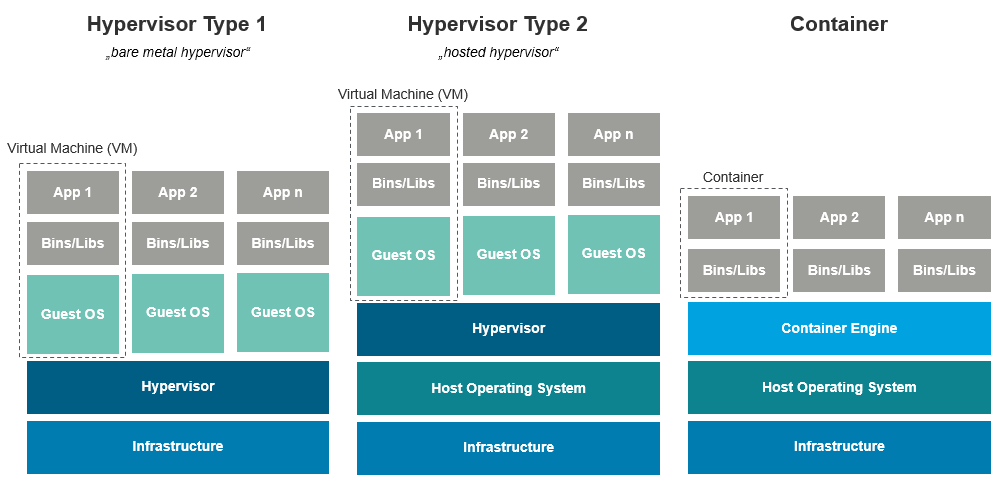
\includegraphics[width=0.95\linewidth]{UNINA_BSc_Final_Report//img//explanation/VM vs Container.png}
    \caption{confronto virtualizzazione e containerizzazione \cite{Vm-vs-Container}}
    \label{fig:Container}
\end{figure}
Un container non è altro che un pacchetto che racchiude del codice software e tutti i componenti necessari per eseguirlo correttamente, come librerie e altre dipendenze, tutte incorporate in una singola struttura. \\
La containerizzazione di un applicazione porta numerosi vantaggi, innanzitutto grazie all'isolamento dell'applicazione quest'ultima potrà essere eseguita in maniera \textbf{indipendente dall'ambiente} in cui si trova, ad esempio a prescindere dal sistema operativo dell'host, ma il principale vantaggio è dato dalla \textbf{portabilità} e \textbf{leggerezza} di questi ultimi, infatti a differenza di una macchina virtuale che può essere vista come un sistema a sé stante, un container invece può essere visto come un'estensione di un classico processo di un sistema operativo e \textbf{non necessita della virtualizzazione delle risorse}, ma lavora direttamente condividendo il Kernel dell'host [fig. \ref{fig:Container}]. \\
Sfruttano tecnologie come i \textit{namespace}, che permettono di isolare un insieme di risorse, e i \textit{cgroups}, che permettono invece di definire e limitare l'utilizzo delle risorse da parte di un gruppo di processi ad esempio di uno stesso namespace. Questo permette di \textbf{ridurre drasticamente l'utilizzo delle risorse} come lo spazio sul disco e in memoria, i tempi di avvio, etc... anche in termini di ordini di grandezza, semplificando la scalabilità di un applicazione.
\\
I container a loro volta non sono altro che delle \textbf{istanze} di quelle che vengono chiamate \textbf{immagini},
definibili come l'analogo delle classi nella programmazione a oggetti, ma queste vengono a loro volta create effettuando un processo di \textbf{build} tramite appositi file di configurazione ed inoltre sarà anche necessario rilasciare e scalare opportunamente tali container. Questo insieme di operazioni dovrebbe poi essere ripetuto per ogni singolo container (che possono facilmente arrivare ad esserne centinaia), ed è per questo scopo che sono nati strumenti come Kubernetes che si occupano di \textbf{automatizzare} tutte queste operazioni.

\subsection{Architettura}
\begin{figure}[ht]
    \centering
    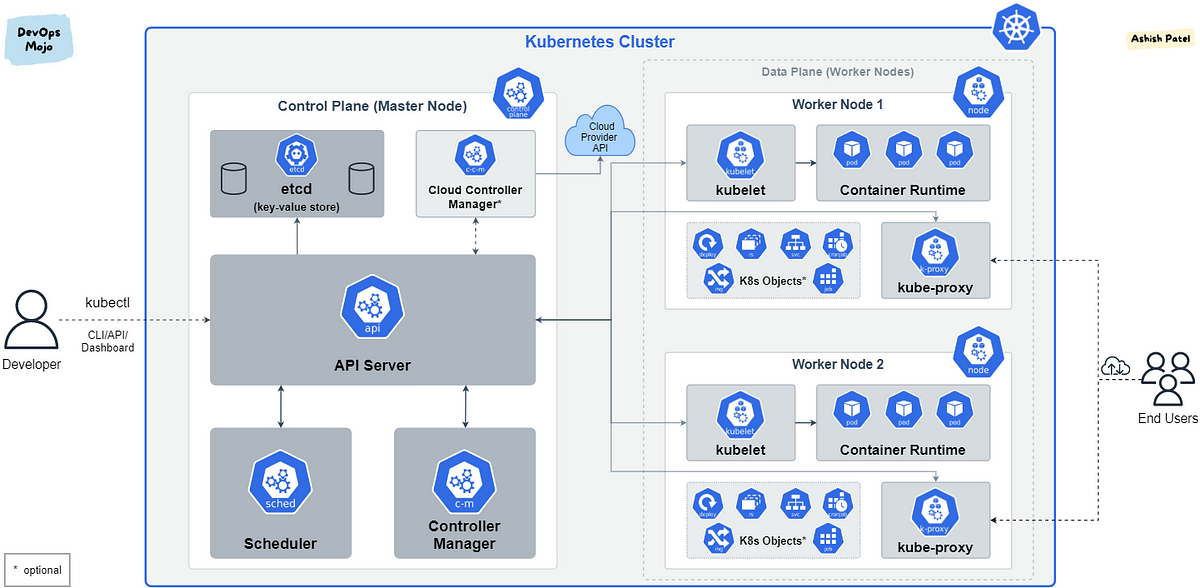
\includegraphics[width=1\linewidth]{UNINA_BSc_Final_Report//img//explanation/kubernetes-cluster-architecture-DevOps.png}
    \caption{architettura di un cluster Kubernetes \cite{k8s-architecture}}
    \label{fig:k8s-architecture}
\end{figure}
Come si può intuire Kubernetes è uno strumento complesso, ed è per questo che per semplificarne lo sviluppo e la comprensibilità è stato suddiviso in diverse componenti coese, raggruppate in quello che viene definito \textbf{cluster} [fig. \ref{fig:k8s-architecture}]: un insieme di macchine comunicanti tra di loro sulla quale vengono eseguite sia tali componenti, sia i container della nostra applicazione.
\\
Un cluster generalmente utilizza uno schema master / worker, ovvero alcune macchine fungeranno da \textbf{Control Plane} (dette \textbf{nodi master}) che si occuperanno di gestire le restanti macchine (dette \textbf{nodi} / \textbf{nodi worker}) sulla quale verranno eseguiti i \textbf{pod} (gruppi di container) ed altre tipologie di \textbf{oggetti} di Kubernetes.
\\
Sia i nodi master che i worker, oltre ad eseguire gli oggetti specifici del sistema che si vuole creare, devono necessariamente eseguire alcune componenti che garantiscono il corretto funzionamento del cluster, ovvero:
\begin{itemize}
    \item \textbf{Control Plane}
        \begin{itemize} 
            \item \textbf{kube-apiserver} \\
            espone le \textbf{API} di Kubernetes e processa le richieste \textbf{REST} o del tool di command line \textbf{kubectl}.
            \item \textbf{etcd} \\
            database persistente, stateful e key-value, contenente tutte le informazioni riguardanti lo stato del cluster.
            \item \textbf{kube-scheduler} \\
            assegna i nuovi pod ai nodi worker in base a diversi criteri.
            \item \textbf{kube-controller-manager} \\
            controlla lo stato desiderato degli oggetti nel cluster e lo confronta con lo stato attuale tramite l'Apiserver, eventualmente applica degli step correttivi per riconciliarli.
        \end{itemize}
    \item \textbf{Nodi}
        \begin{itemize} 
            \item \textbf{kubelet} \\
            intermediario tra l'Apiserver e il nodo, seguendo le istruzioni del nodo master avvia e controlla i pod nei nodi worker.
            \item \textbf{container runtime} \\
            motore per scaricare, eseguire e gestire i container nei pod.
            \item \textbf{kube-proxy} \\
            network proxy che si occupa della gestione delle comunicazioni con i pod internamente ed esternamente.
        \end{itemize}
\end{itemize}
Tutte queste componenti sono \textbf{stateless} e \textbf{comunicano indirettamente} tra di loro utilizzando l'Etcd, ma solo l'Apiserver può accederci e quindi la comunicazione avviene unicamente tramite l'invocazione delle apposite API. \\
Questo pattern rende l'Etcd un \textbf{componente critico}, ed è proprio su tale criticità che è stata basata la campagna di fault/error injection, dove le iniezioni sono state effettuate proprio nella comunicazione tra Apiserver e Etcd.

%*******************************************************************************************************%

\section{Perché Prometheus?}
\textbf{Prometheus} \cite{Prometheus} è un framework di \textbf{monitoraggio} e \textbf{alerting} ormai maturo, che mette a disposizione numerose funzionalità extra come l' immagazzinamento dei dati in maniera persistente, un apposito linguaggio di interrogazione sui dati, etc... che verranno approfondite nel prossimo capitolo.
\\
Ma la vera differenza con i suoi competitor è del far parte della CNCF \cite{CNCF}, perché essendo un progetto open source la sua grande diffusione permette di creare una vasta \textbf{community} attiva, di fondamentale importanza dato che chiunque può realizzare una propria fork del progetto, chiunque può creare dei nuovi moduli per monitorare sistemi e strumenti non ufficialmente supportati (basta dare una rapida occhiata alle loro liste \cite{Prometheus-clients-exporters-list} per vedere come la maggioranza siano sviluppate dalla community), gli aggiornamenti sono continui, le vulnerabilità vengono rilevate e corrette rapidamente e soprattutto la \textbf{documentazione} che si può trovare online è immensamente maggiore rispetto a molte sue alternative. \\
In realtà infatti potremmo dire che Prometheus non abbia dei veri e propri competitor considerata la sua community, ma bensì che esistano delle soluzioni alternative che si focalizzano su specifici obbiettivi, ad esempio per citarne alcune:
\begin{itemize}
    \item \textbf{InfluxDB} \cite{InfluxDB}: particolarmente efficiente in termini di risorse, ha un linguaggio di interrogazione più semplice da utilizzare e più rapido, ma ha un ecosistema decisamente più acerbo e risulta essere più complesso da configurare.
    \item \textbf{Graphite} \cite{Graphite}: punta tutto sulla semplicità di configurazione e d'uso, ma allo stesso tempo ha meno funzionalità di interrogazione e non è molto adatto per ambienti di monitoraggio complessi.
    \item \textbf{VictoriaMetrics} \cite{VictoriaMetrics}: probabilmente l'alternativa che più si avvicina a Prometheus, infatti può essere vista come una sua variante ma con l'obiettivo di avere un footprint minore ed offre anche un linguaggio di interrogazione più avanzato, ma al costo di avere meno funzionalità ed un ecosistema decisamente meno maturo, quindi con documentazione online e supporto della community inferiore.
\end{itemize}
Quindi anche se esistono numerose altre alternative, analogamente a quanto successo con Kubernetes, anche Prometheus è diventato un de facto standard nel suo ambiente.
\chapter{Prometheus} \label{chap:Prometheus}

\section{Cosa è?}
\textbf{Prometheus} è un framework di \textbf{monitoraggio} e di \textbf{alerting} che può essere utilizzato sia per il monitoraggio dello stato di salute di un cluster sia per il monitoraggio di una specifica applicazione. Sulle \textbf{metriche} prodotte è anche possibile applicare delle \textbf{regole} di alerting per segnalare eventuali criticità su diversi canali di comunicazione come email, slack, etc... \\
Inizialmente sviluppato da SoundCloud \cite{SoundCloud}, anche questo strumento è stato poi donato alla CNCF \cite{CNCF} e reso open source, diventando uno degli strumenti più diffusi nella sua categoria soprattutto grazie al suo \textbf{approccio modulare} che permette a chiunque lo desideri, di creare nuovi moduli per monitorare sistemi / strumenti / etc... non ufficialmente supportati.


\section{Metriche}
I dati utilizzati da Prometheus sono rappresentati sotto forma di metriche chiamate \textbf{time series}, composte da un \textbf{timestamp} relativo all'istante di collezionamento (nel tempo per una stessa metrica avremo più rilevamenti), e da coppie key-value opzionali dette \textbf{label} utilizzate per categorizzarle. \\
Queste time series possono essere facilmente interrogate e manipolate tramite l'apposito linguaggio di interrogazione detto \textbf{PromQL} \cite{Prometheus-query-language}, standardizzandone l'accesso e rendendo possibile interrogare tali metriche da diversi strumenti come la web UI di Prometheus, da richieste HTTP oppure tramite tool di terze parti come \textbf{Grafana} \cite{Grafana}. Grafana in particolare permette di creare \textbf{dashboard e grafi personalizzati} tramite un'apposita web UI, velocizzando la valutazione dello stato del sistema. 

\section{Architettura}
\begin{figure} [ht]
    \centering
    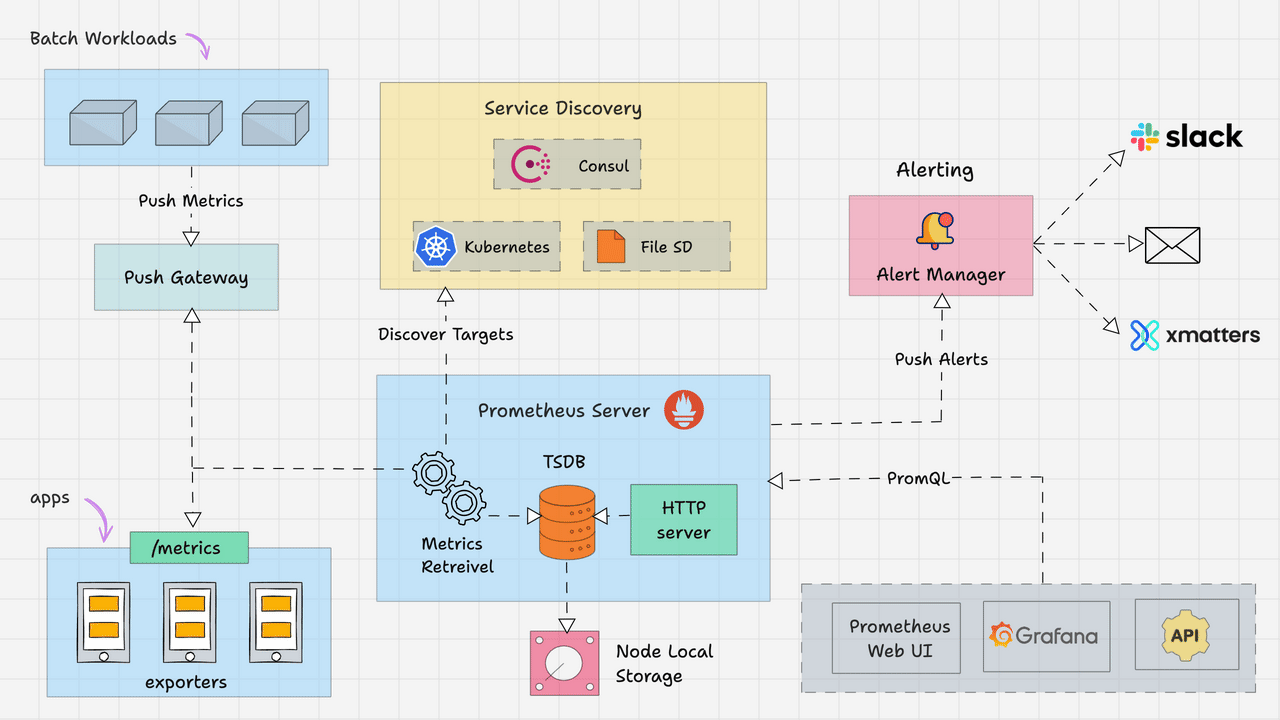
\includegraphics[width=1\linewidth]{UNINA_BSc_Final_Report//img//explanation/prometheus-architecture.png}
    \caption{architettura framework Prometheus \cite{Prometheus-architecture}}
    \label{fig:prometheus-architecture}
\end{figure}
L'approccio utilizzato da Prometheus per recuperare i dati è detto \textbf{scraping}, che sarà approfondito a breve, mentre i dati come già detto sono rappresentati sotto forma di metriche.\\ 
L'architettura si può suddividere nelle seguenti componenti, considerabili come moduli a se stanti [fig. \ref{fig:prometheus-architecture}]: \\

\begin{itemize}
    \item \textbf{Server} \\
    cuore di questo strumento, colleziona le metriche dai vari target con un pattern pull, periodicamente tramite richieste HTTP (processo detto \textbf{scraping}), dove il periodo di tempo può essere personalizzato. E' composto a sua volta da:
    \begin{itemize} 
        \item \textbf{Time-Series Database (TSDB)}: database che immagazzina le time series delle metriche in maniera persistente ed efficiente, sfruttando apposite policy temporali per la conservazione; di default salva i dati in locale sul nodo in cui viene installato Prometheus, ma può essere configurato per il salvataggio in cloud.
        \item \textbf{HTTP server}: abilita l'interrogazione al TSDB tramite richieste HTTP ricevute dall'esterno contenenti le query in \textit{PromQL}.
        \item \textbf{Metrics Retrieval}: colleziona le metriche dai \textbf{target} inviando richieste HTTP periodicamente.
    \end{itemize}

    \item \textbf{Targets} \\
    sorgenti per lo scraping del server, in genere utilizzano degli \textbf{exporter} che convertono delle metriche da un formato non supportato (per esempio metriche di sistema) ad uno adatto a Prometheus, o delle \textbf{librerie cliente} che permettono di esporre delle metriche personalizzate da un applicazione scrivendo direttamente nel codice. Entrambe queste tipologie di moduli possono essere creati da zero da qualsiasi utente, per questo le loro liste vengono suddivise in ufficiali e non \cite{Prometheus-clients-exporters-list}. \\
    Negli scenari in cui non è possibile utilizzare il pattern pull come in task di breve durata, allora si può utilizzare il \textbf{PushGateway}, un componente a se stante che funge da buffer temporaneo, permettendo ai target di inviare direttamente le metriche (pattern \textbf{push}) a quest'ultimo, dalla quale saranno poi estratte come in un target classico.

    \item \textbf{Service Discovery} \\
    uno dei concetti principali di questo strumento, i target possono essere rilevati in 2 modi: 
    \begin{itemize} 
        \item \textbf{configurazione statica}: i target sono hard coded nei file di configurazione di Prometheus o in appositi file YAML/Json, ma ciò è possibile solo con target che hanno endpoint statici, che in genere non è nella natura degli oggetti di Kubernetes.
        \item \textbf{Sevice Discovery}: consente a Prometheus di rilevare e monitorare automaticamente i target senza richiedernee la configurazione manuale per ognuno di essi.
    \end{itemize}

    \item \textbf{Alert Manager} \\
    per quanto riguarda l'alerting, Prometheus si occupa unicamente di \textbf{triggerare} gli alert definendo delle \textbf{treshold}, ma tali alert sono poi gestiti dall'\textbf{Alert Manager}, il quale dopo averci effettuato diverse manipolazioni come la decuplicazione, raggruppamento, etc... notificherà gli appositi destinatari in base ai diversi criteri di \textbf{routing} con il quale è stato configurato.
    
\end{itemize}

\section{Prometheus Operator} 
Per installare Prometheus si possono usare 2 approcci principalmente, uno \textbf{classico} installando il framework come una normale applicazione usando dei file binari pre-compilati, delle immagini Docker o Helm, dove però è richiesto un processo di configurazione lento e tedioso consistente nella creazione e modifica di diversi file di configurazione in maniera statica, aumentando di molto i tempi di setup ed eventualmente di troubleshooting. \\
Invece, un altro approccio che si può utilizzare è quello di sfruttare gli \textbf{operatori} di Kubernetes, che potremo dire essere la nuova frontiera per la distribuzione di applicazioni in un cluster, infatti gli operatori non sono altro che delle \textbf{estensioni} che permettono di integrare un'applicazione in maniera più stretta con Kubernetes, dando così la possibilità di creare degli \textbf{oggetti personalizzati} utilizzando delle \textbf{Custom Resource Definitions} (CRDs). 
\\
Prometheus mette a disposizione il \textbf{Prometheus Operator} \cite{Prometheus-operator}, che consente di installare in modo semplice l'intero stack di monitoraggio (Prometheus, Alert Manager, Grafana, etc.), semplificando significativamente la configurazione del framework. Grazie a questo strumento, non è più necessario modificare manualmente i file di configurazione, ma si possono invece creare oggetti personalizzati, come il Deployment di Prometheus o dell'Alert Manager. La configurazione può essere suddivisa in più oggetti personalizzati distinti, evitando l'uso di un unico file. Ad esempio, il ServiceMonitor permette di dichiarare quali servizi di Kubernetes monitorare, migliorando la modularità e la gestione della configurazione. \\
Tutto ciò avviene semplicemente installando il Prometheus Operator e creando nuovi oggetti personalizzati, che verranno automaticamente rilevati tramite l'uso delle label, aggiornando automaticamente tutte le configurazioni che in passato avrebbero richiesto interventi manuali.

\section{Sistema locale}

Come già anticipato per comprendere al meglio il funzionamento di tali strumenti, è stato ricreato un ambiente simile a quello utilizzato nella campagna di fault/error injection con un'applicazione campione [fig. \ref{fig:local-cluster}], con ovvie limitazioni a causa della disponibilità di risorse computazionali. 

\begin{figure} [ht]
    \centering
    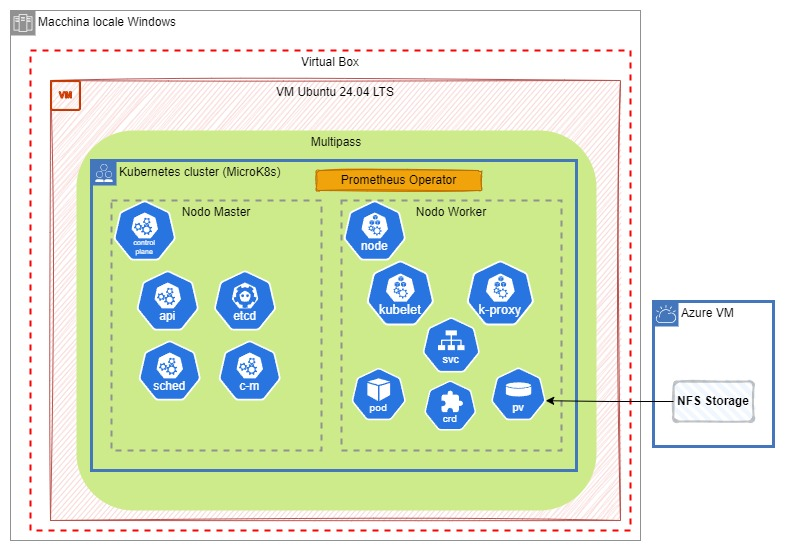
\includegraphics[width=1\linewidth]{UNINA_BSc_Final_Report//img//explanation/local_environment.jpg}
    \caption{infrastruttura cluster locale}
    \label{fig:local-cluster}
\end{figure}

\subsection{Ambiente}
Partendo dall'alto verso il basso il sistema gira su una macchina virtuale Ubuntu 24.04 LTS \cite{Ubuntu} eseguita su VirtualBox 7.0.20 \cite{VirtualBox}, con 4 core e circa 10 GB di memoria. \\
Su tale VM gira l'intero cluster, composto da 2 nodi (1 master e 1 worker), dove ogni nodo corrisponde a sua volta ad un altra macchina virtuale Ubuntu 24.04 LTS da 1 core e 4 GB di memoria, gestite con Multipass 1.14.0 \cite{Multipass}.

\subsection{MicroK8s}
Per creare un cluster Kubernetes è stato utilizzato \textbf{MicroK8s} 1.30.0 \cite{MicroK8s}, framework open source che permette di creare un \textbf{cluster lite} adatto a sistemi con poche risorse. \\
Il vero vantaggio di tale framework però è nella \textbf{semplicità} della configurazione del cluster, il punto debole di Kubernetes, infatti MicroK8s permette di creare un cluster semplicemente installando il framework su ogni nodo (ad esempio con \textbf{Snap} \cite{Snap}), utilizzare un apposito comando dal nodo master e copiare ed incollare le istruzioni a schermo sui nodi worker, ed il cluster è già configurato. \\
Un altre grande vantaggio di MicroK8s sono gli \textbf{addon}, ovvero delle estensioni attivabili direttamente tramite MicroK8s già preconfigurate e pronte all'uso, in particolare è stato abilitato l'addon \textbf{observability} che permette di installare lo stack \textbf{Kube-prometheus} \cite{Kube-prometheus}, che comprende il Prometheus Operator, Grafana, l'Alert Manager e un insieme di exporter per monitorare lo stato del cluster come Kube-state-metrics \cite{Kube-state-metrics} e node-exporter \cite{Node-exporter}. Anche in questo caso con un semplice comando da terminale \textit{microk8s enable observability}, l'intero ecosistema di Prometheus è già in funzione per monitorare lo stato del cluster con anche delle regole di alerting predefinite.

\subsection{Applicazione campione}
Come applicazione da monitorare è stata scelta un'applicazione per la gestione di sensori di temperatura e pressione, costituita da un BE in Flask e da degli script per simulare le richieste dei client \footnote{Il codice è disponibile su GitHub \cite{github-repo}, mentre le immagini dei container su DockerHub \cite{docker-images}}.
Oltre a monitorare lo stato del cluster, è stata modificata l'applicazione utilizzando una delle client library di Prometheus permettendo di aggiungere l'endpoint per lo scraping e realizzare delle metriche personalizzate [fig. \ref{fig:flask-be}] per monitorare le richieste ricevute, il tempo di elaborazione e le relative risposte.


\begin{figure} [ht]
    \centering
    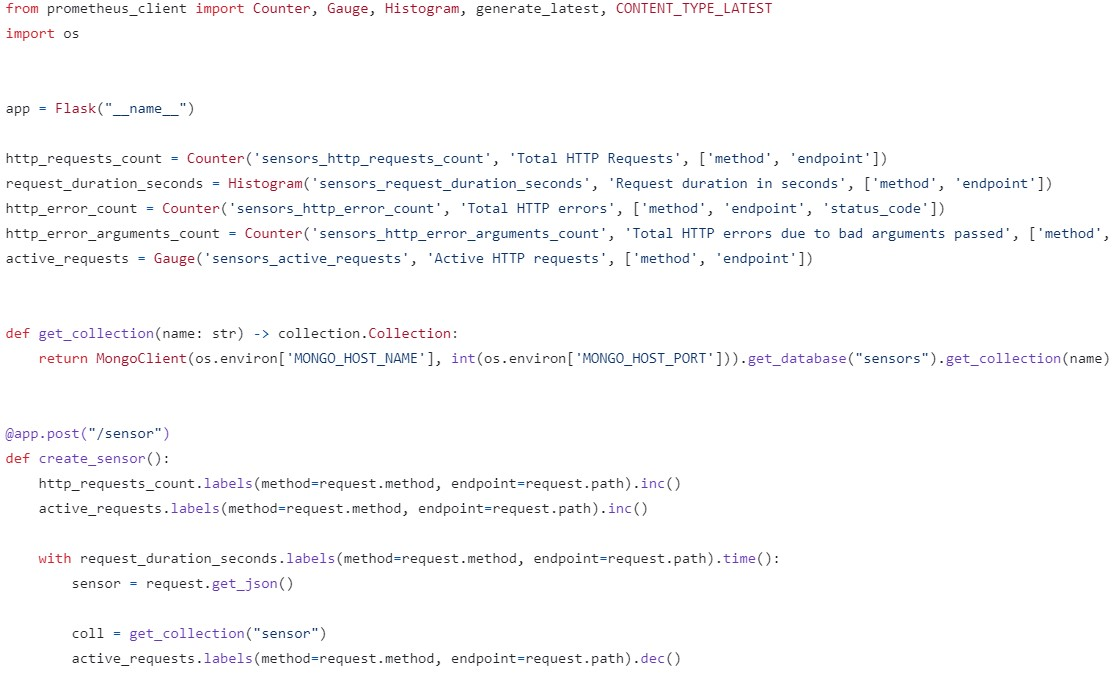
\includegraphics[width=0.95\linewidth]{UNINA_BSc_Final_Report//img//explanation/controller_example.jpg}
    \caption{esempio BE Flask con metriche da client library}
    \label{fig:flask-be}
\end{figure}

\subsection{Configurazione applicazione campione}
Per poter monitorare anche l'applicazione d'esempio è necessario creare degli appositi oggetti di Kubernetes \footnote{Tutti i file per creare questi oggetti sono disponibili sul repository GitHub \cite{github-repo} in formato .yaml.} , sia per quanto riguarda la gestione dell'applicazione che per configurare Prometheus ad effettuare lo scraping delle nuove metriche.

\subsubsection{Deployment applicazione}
Il deploy dell'applicazione è costituito dai seguenti oggetti Kubernetes:
\begin{itemize}
    \item \textbf{Deployment} del BE in Flask.
    \item \textbf{Service} \footnote{I Service sono degli oggetti di Kubernetes che si occupano di rendere disponibile in rete determinati pod, selezionati ad esempio tramite label, e fare loro da load balancer.} per esporre il BE all'esterno.
    \item \textbf{StatefulSet} per l'istanza di MongoDB.
    \item \textbf{Service} per esporre MongoDB al BE.
    \item \textbf{PersistentVolume} per rendere persistenti i dati di MongoDB, utilizzando una macchina virtuale su Azure come NFS storage.
    \item \textbf{Deployment} per gli script dei client.
\end{itemize}

\subsubsection{Configurazione Prometheus}
La configurazione di Prometheus è avvenuta in maniera analoga a quanto fatto precedentemente grazie al Prometheus Operator, con il quale è stato sufficiente creare degli \textbf{oggetti personalizzati} per tale operatore senza dover toccare i file di configurazione di Prometheus stesso. Per fare ciò è stato sufficiente creare un numero ridotto di oggetti sfruttando gli oggetti già creati dall'addon observability, impostando le \textbf{label} dei nuovi oggetti in maniera opportuna per far funzionare correttamente il \textbf{service discovery} di Prometheus. In particolare:
\begin{itemize}
    \item \textbf{Service} per esporre Prometheus, Grafana e l'Alert Manager all'esterno.
    \item \textbf{ServiceMonitor} per abilitare il monitoraggio (scraping) al Service del BE.
    \item \textbf{PrometheusRule} per creare un'alert rule personalizzata campione.
\end{itemize}

Con questa configurazione possiamo sia monitorare lo stato del cluster sfruttando gli exporter e le dashboard preinstallate [fig. \ref{fig:grafana-cluster}] o sfruttando metriche e dashboard personalizzate [fig. \ref{fig:grafana-sensor}], sia applicare delle regole di alerting in pochi semplici passaggi.
\\
\begin{figure} [ht]
    \centering
    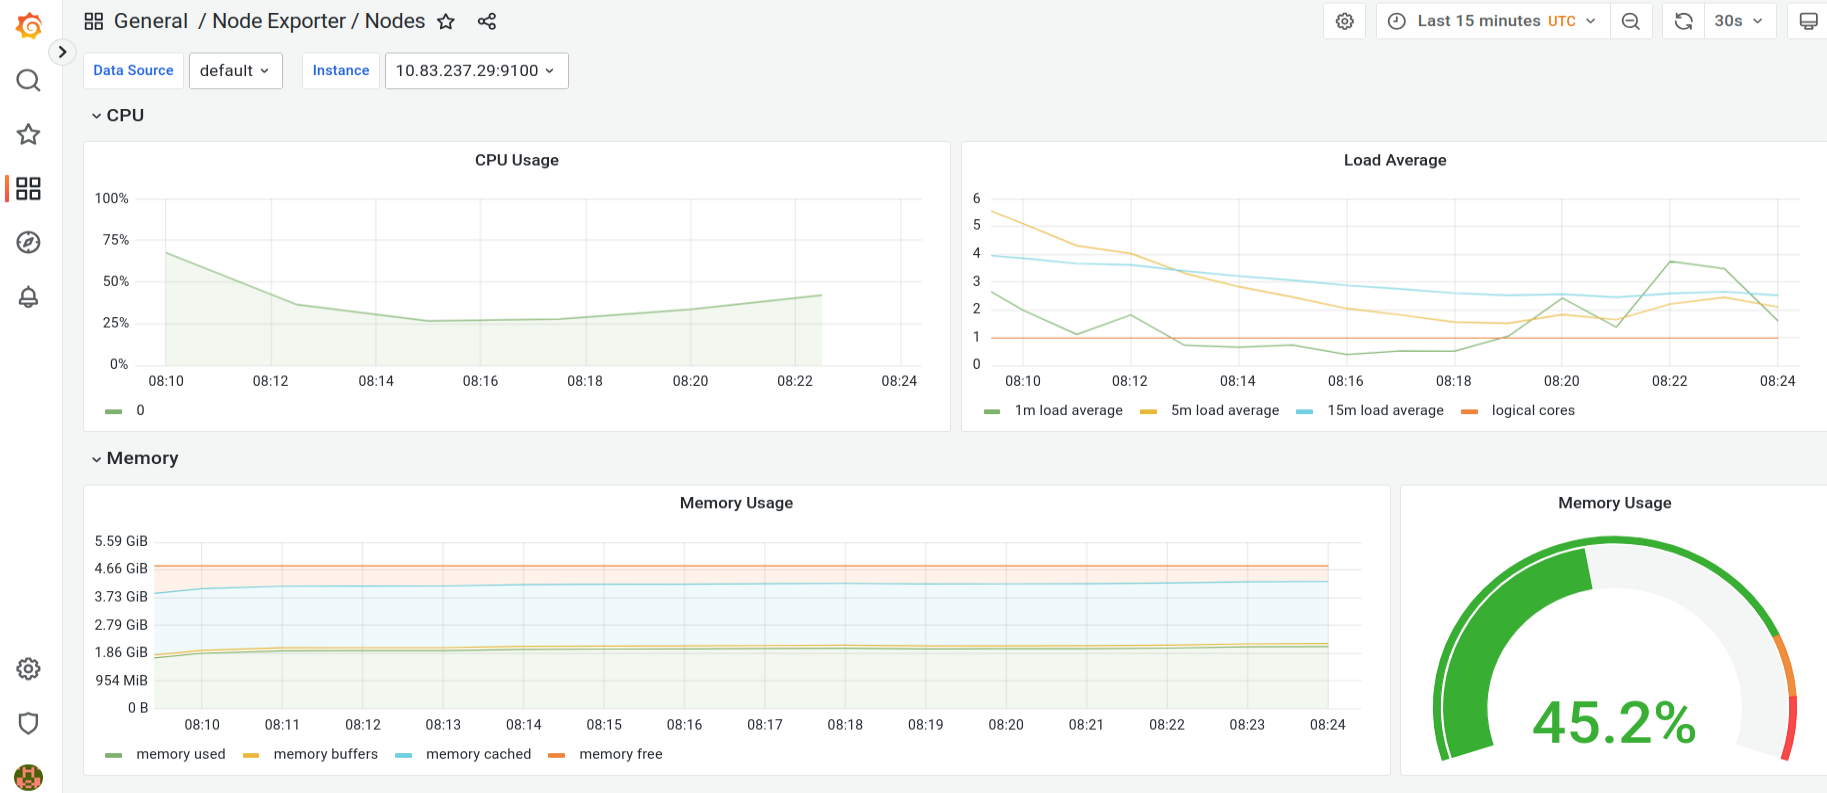
\includegraphics[width=1\linewidth]{UNINA_BSc_Final_Report//img//explanation/grafana_example_white.png}
    \caption{dashboard Grafana con metriche da Node Exporter}
    \label{fig:grafana-cluster}
\end{figure}

\begin{figure} [ht]
    \centering
    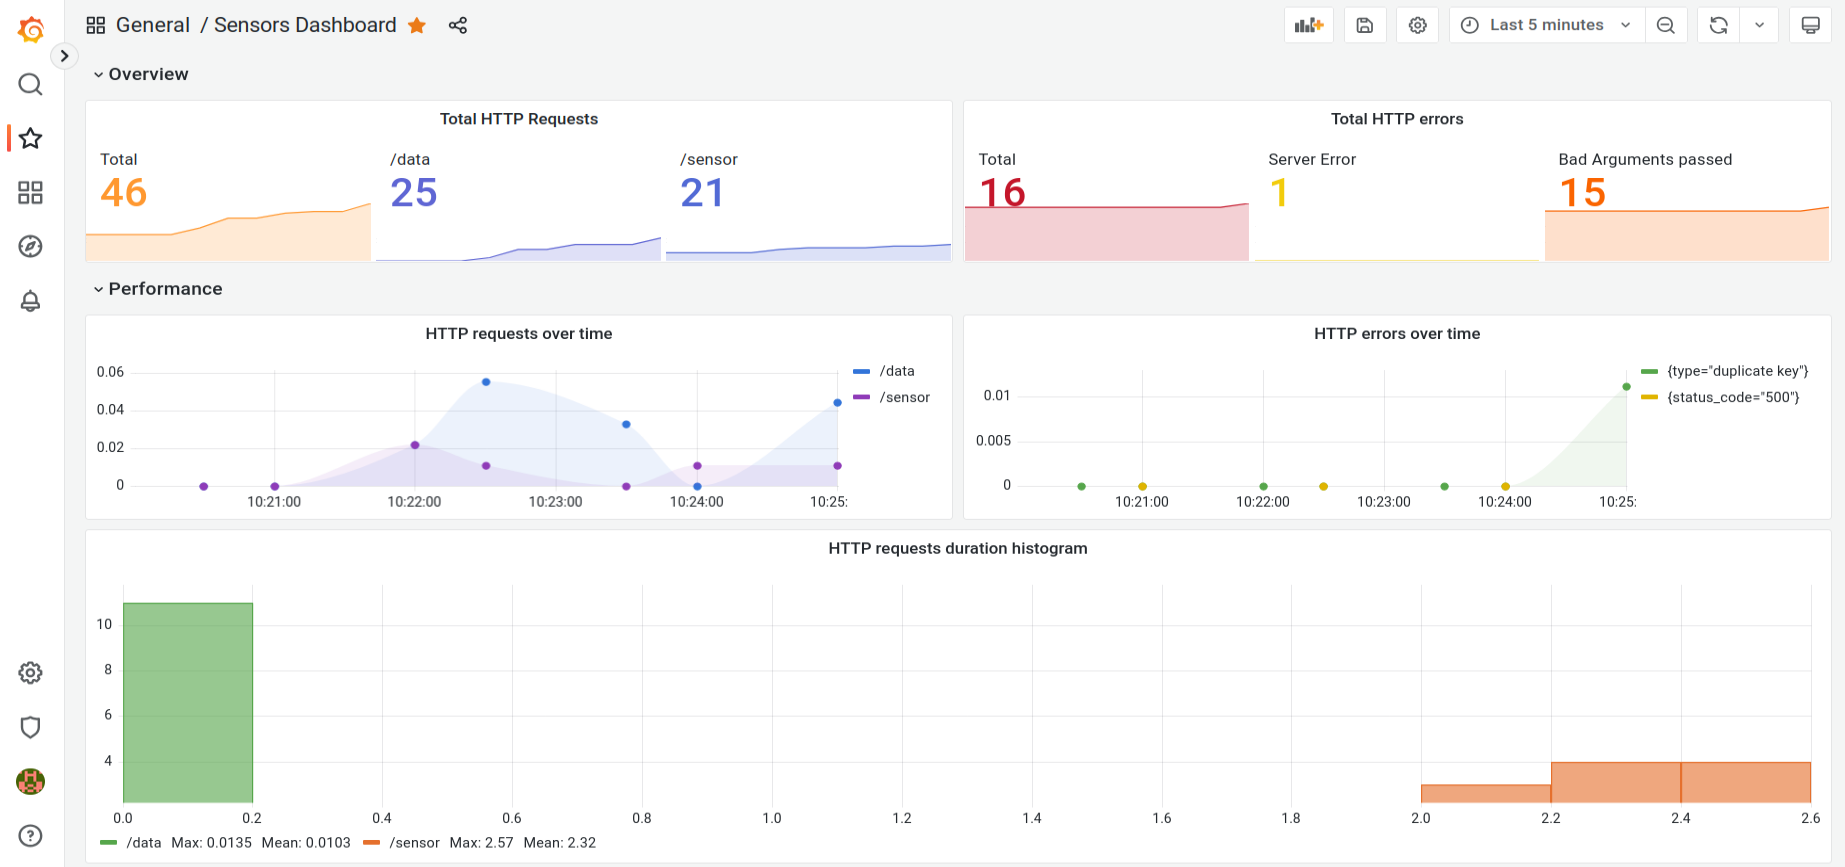
\includegraphics[width=1\linewidth]{UNINA_BSc_Final_Report//img//explanation/grafana_sensor_example_white.png}
    \caption{dashboard Grafana personalizzata del BE}
    \label{fig:grafana-sensor}
\end{figure}
\chapter{Analisi dataset} \label{chap:Dataset}
In questa seconda parte l'obiettivo è quello di ricercare una correlazione tra gli errori scatenati durante la campagna di fault/error injection e le metriche estratte da Prometheus, in maniera tale da mostrare come sia possibile utilizzare tali metriche per creare apposite regole di alerting e far attivare tempestivamente eventuali operazioni di troubleshooting.


\section{Dataset}
\subsection{Campagna injection}
La campagna di fault/error injection è stata condotta utilizzando \textbf{Mutiny}, un framework appositamente sviluppato per Kubernetes che consente di manipolare i messaggi scambiati tra le varie componenti del sistema. L'applicazione monitorata è un web server Flask, il quale risponde alle richieste dei client eseguendo elaborazioni casuali. Le manipolazioni dei messaggi possono avvenire durante la comunicazione \textbf{tra l'Apiserver e l'Etcd}, con la possibilità di influire direttamente sullo stato attuale o desiderato del cluster, oppure \textbf{tra le componenti e l'Apiserver}, sebbene in quest'ultimo caso sia più probabile che i messaggi vengano identificati come corrotti e rigettati dall'Apiserver stesso.
\\
Durante la campagna sono state eseguite tre principali tipologie di iniezione:
\begin{itemize} 
    \item \textbf{Bit flip}: viene invertito un singolo bit all'interno del messaggio. 
    \item \textbf{Data-type set}: viene impostato un valore boundary o errato, a seconda del tipo di campo interessato.
    \item \textbf{Message drop}: simula la mancata ricezione di un aggiornamento di stato del cluster, dovuta a vari motivi come richieste fallite, bug, etc...
\end{itemize}
Per garantire un dataset completo, le metriche di Prometheus sono state raccolte utilizzando node exporter \cite{Node-exporter}, kube-state-metrics \cite{Kube-state-metrics} e metriche personalizzate dell'applicazione. Queste metriche sono state ricavate per ogni singola esecuzione della campagna. In particolare, sono state effettuate 300 run di controllo (\textit{gold runs}), dai cui risultati sono stati estratti i valori di riferimento per confrontare le time series generate durante le 8.782 run di iniezione.


\subsection{Struttura dataset}
 La combinazione di metriche ottenute durante la campagna permette di estrarre informazioni riguardanti lo stato dei nodi, degli oggetti Kubernetes e dell'applicazione, offrendo una vista completa sullo stato di salute del sistema.
\\
I dati sui cui sono state effettuate le analisi però sono solo un subset dell'intero dataset della campagna, con un numero limitato di tipologie di metriche e di classi di dati.

\subsection{Classificazione}
Per poter effettuare un'analisi in maniera più sistematica, i risultati delle run durante la campagna sono stati classificati a seconda del tipo di errore \textbf{visto dall'utente}:

\begin{itemize}
    \item Nessun Impatto Significante (\textbf{NSI}).
    \item Higher Response Time (\textbf{HRT}), solo ritardi temporali.
    \item Intermittent Availability (\textbf{IA}), risposte di errore a intermittenza.
    \item Service Unreachable (\textbf{SU}), servizio irraggiungibile.
\end{itemize}
a seconda del tipo di errore al \textbf{livello di orchestrazione}, di cui nel subset sono presenti:
\begin{itemize}
    \item \textbf{LeR}: il numero di repliche pronte, Pod creati o endpoint è stabile e inferiore alla baseline.
    \item \textbf{MoR}: il numero di repliche pronte, Pod creati o endpoint è superiore alla baseline.
    \item \textbf{Net}: il numero di repliche pronte e Pod è corretto, ma alcuni non sono raggiungibili o utilizzati nel bilanciamento del carico.
\end{itemize}
ed a seconda di sotto quale tipologia di \textbf{workload} di orchestrazione si è verificato l'errore:
\begin{itemize}
    \item \textbf{Deploy}: crea nuovi Deployment e Pod correlati.
    \item \textbf{Scale}: aumenta il numero di repliche dei Deployment esistenti. 
    \item \textbf{Failover} / \textbf{Availab}: forza i pod ad essere rigenerati tramite l'iniezione di un errore.
\end{itemize}

\begin{figure} [ht]
    \centering
    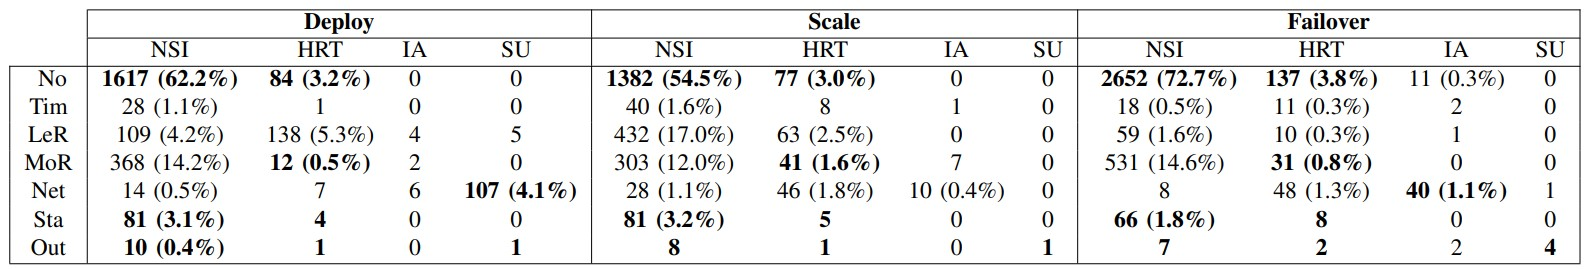
\includegraphics[width=1\linewidth]{UNINA_BSc_Final_Report//img//explanation/failure_full_map.jpg}
    \caption{risultati campagna di injection mappati errori - workload}
    \label{fig:of-cf-map}
\end{figure}

\section{Analisi}
L'approccio scelto per analizzare le metriche di Prometheus a disposizione è quello di realizzare dei grafi che permettano di visualizzare l'andamento delle metriche nei diversi scenari di errore a livello orchestrazione e per tipologia di workload. \\
Per fare ciò è stato realizzato un \textbf{notebook Jupyter} \cite{Jupyter}, che permette di caricare il dataset in memoria per poi scegliere singolarmente quali grafi realizzare in un secondo momento. Questo è possibile in quanto il flusso per generare un grafo è composto da 3 step separati: il caricamento del dataset in memoria, l'elaborazione dei dati per semplificarne l'utilizzo ed infine la generazione del grafo. \footnote{il notebook intero è reperibile sul repository GitHub \cite{github-repo}}

\subsection{Codice}
\subsubsection{Caricamento dati}

Nel dataset le metriche seguono circa questa struttura: \\  
/\textit{tipo errore orchestrazione}/\textit{[num. run]\_workload}/\textit{file metrica} \\
quindi per caricare i dati viene esplorato l'intero albero di directory, estrapolando i valori dai file delle metriche, file per file, per ottenere un array JSON [fig. \ref{fig:code-load-data}], dove una possibile riga è:
\begin{footnotesize}
\begin{verbatim}
{
    'metric': 
        {
            '__name__': 'node_memory_MemFree_bytes', 
            'instance': '192.168.100.20:9100'
        },
    'value': [1695843909.839, '1976422400'],
    'condition': 'Baselines', 'workload': 'deploy'
}
\end{verbatim}
\end{footnotesize}
in cui possiamo osservare il tipo di metrica, la time series (timestamp + valore), se la time series fa parte di una gold run o di una delle run di iniezione e sotto quale workload è stata rilevata.
\begin{figure} [ht]
    \centering
    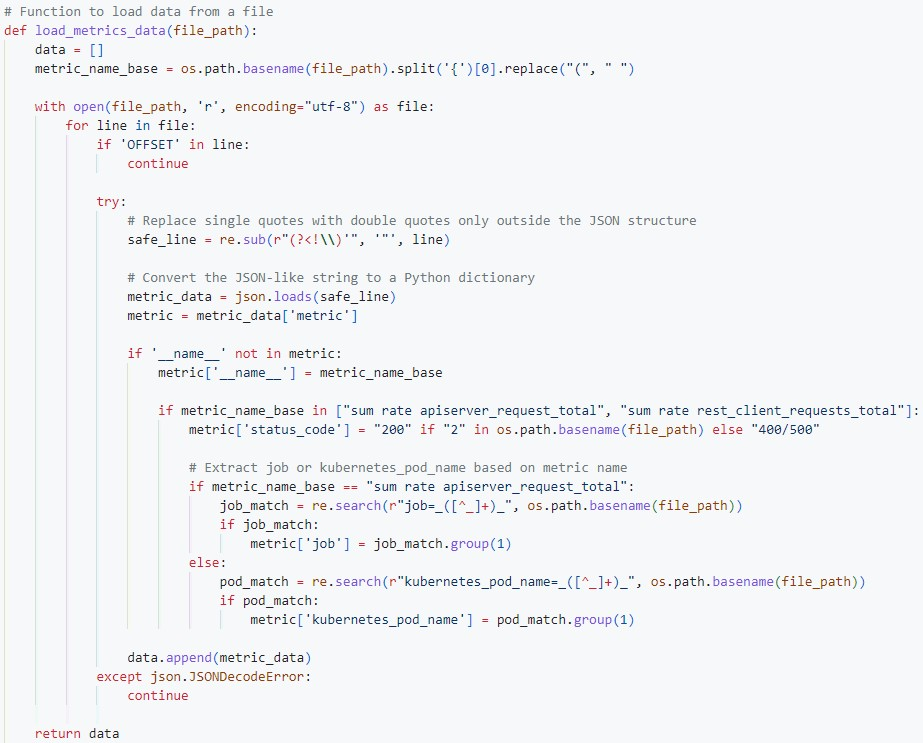
\includegraphics[width=0.8\linewidth]{UNINA_BSc_Final_Report//img//explanation/code_load_data.jpg}
    \caption{estrazione metrica in JSON}
    \label{fig:code-load-data}
\end{figure}

\subsubsection{Elaborazione dati}
Per poter lavorare più facilmente con i dati, l'array JSON viene convertito in un Dataframe della libreria Pandas \cite{code-pandas} [fig. \ref{fig:code-dataframe}], libreria che offre strutture dati e metodi per manipolare i dati.

\begin{figure} [ht]
    \centering
    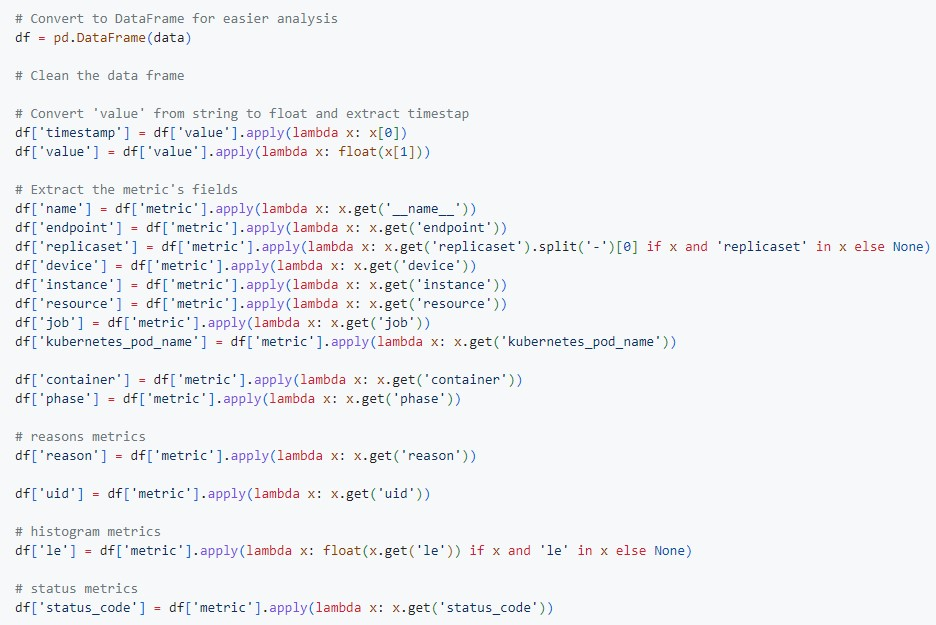
\includegraphics[width=0.9\linewidth]{UNINA_BSc_Final_Report//img//explanation/code_dataframe.jpg}
    \caption{conversione array JSON in Dataframe}
    \label{fig:code-dataframe}
\end{figure}

\subsubsection{Generazione grafi}
La generazione dei grafi avviene utilizzando la libreria \textbf{Matplotlib} \cite{code-matplotlib} e il suo toolkit \textbf{Seaborn} \cite{code-seaborn}, che semplifica la creazione dei grafi più comuni ed è compatibile con le funzionalità della libreria Pandas, grazie alle quali è stato possibile realizzare boxplot e heatmap [fig. \ref{fig:code-boxplot}].
\begin{figure} [!ht]
    \centering
    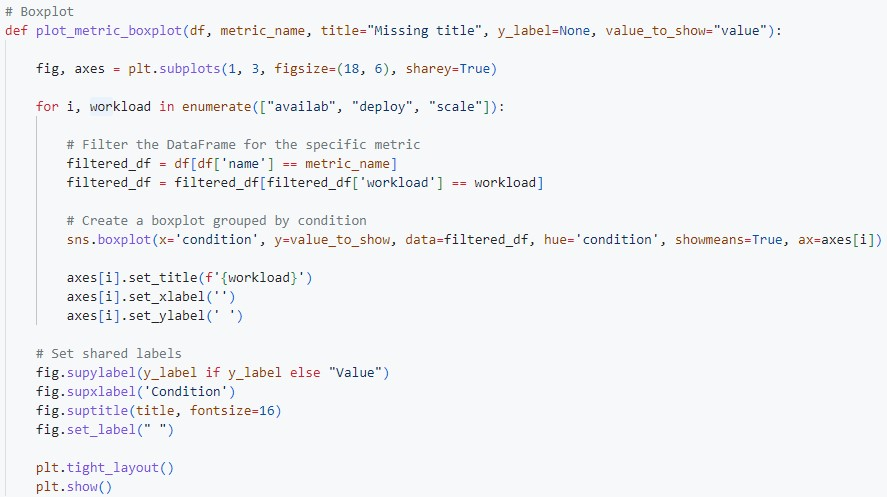
\includegraphics[width=0.9\linewidth]{UNINA_BSc_Final_Report//img//explanation/code_boxplot.jpg}
    \caption{codice boxplot}
    \label{fig:code-boxplot}
\end{figure}

\subsubsection{Boxplot e Heatmap} 
I box plot sono strumenti grafici utili per visualizzare la distribuzione di un insieme di dati. La scatola nel grafico rappresenta l'\textbf{intervallo interquartile} (\textbf{IQR}), con la linea centrale che indica la mediana, mentre i \textit{whisker} si estendono fino ai valori minimo e massimo, a meno che questi non siano considerati \textit{outlier} (valori anomali) [fig. \ref{fig:plot-boxplot-example}]. Questo tipo di grafico consente di identificare eventuali variazioni nell'andamento delle metriche in funzione della tipologia di errore e del carico di lavoro, permettendo un confronto chiaro delle diverse distribuzioni.

\begin{figure} [ht] \centering 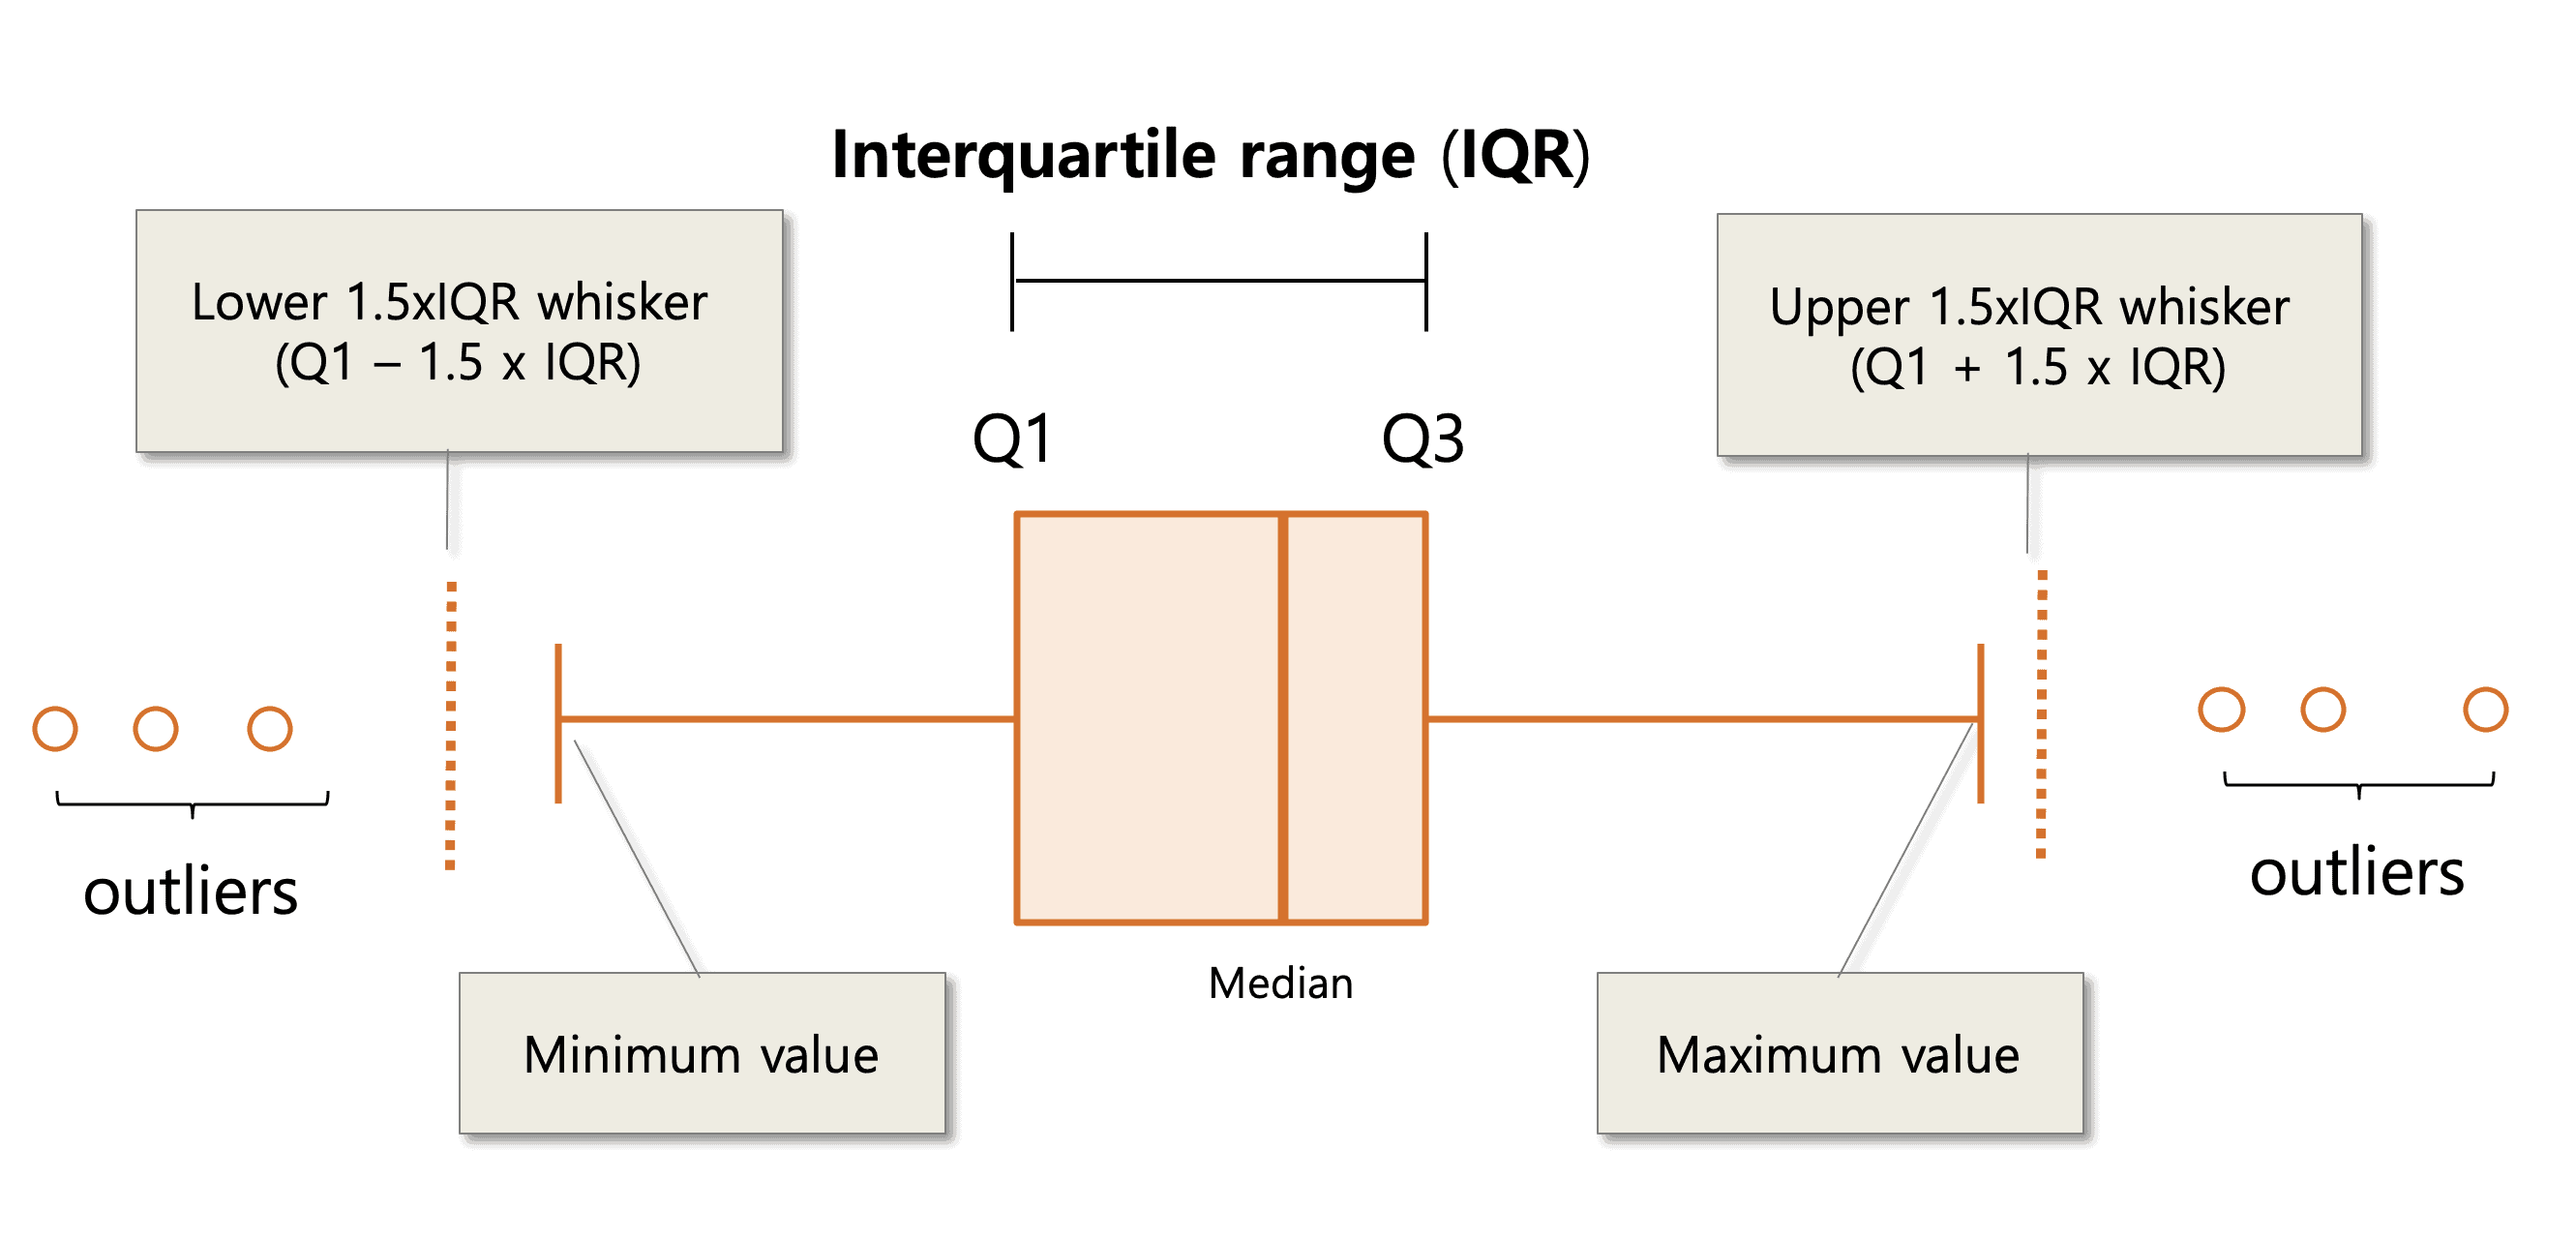
\includegraphics[width=1\linewidth]{UNINA_BSc_Final_Report//img//plots/boxplot-example.png} \caption{esempio di box plot \cite{boxplot-example}} \label{fig:plot-boxplot-example} 
\end{figure}

Le heatmap, invece, sono rappresentazioni grafiche che utilizzano una \textbf{scala di colori} per visualizzare la densità dei dati all'interno di un'area specifica. Nel contesto di questo lavoro, le aree rappresentano combinazioni tra il tipo di errore a livello di orchestratore e la tipologia di workload. Le zone con colori più intensi (zone "calde") indicano una maggiore concentrazione di dati, facilitando così l'individuazione di pattern o anomalie nelle distribuzioni [fig. \ref{fig:plot-heatmap-example}].

\begin{figure} [ht] \centering 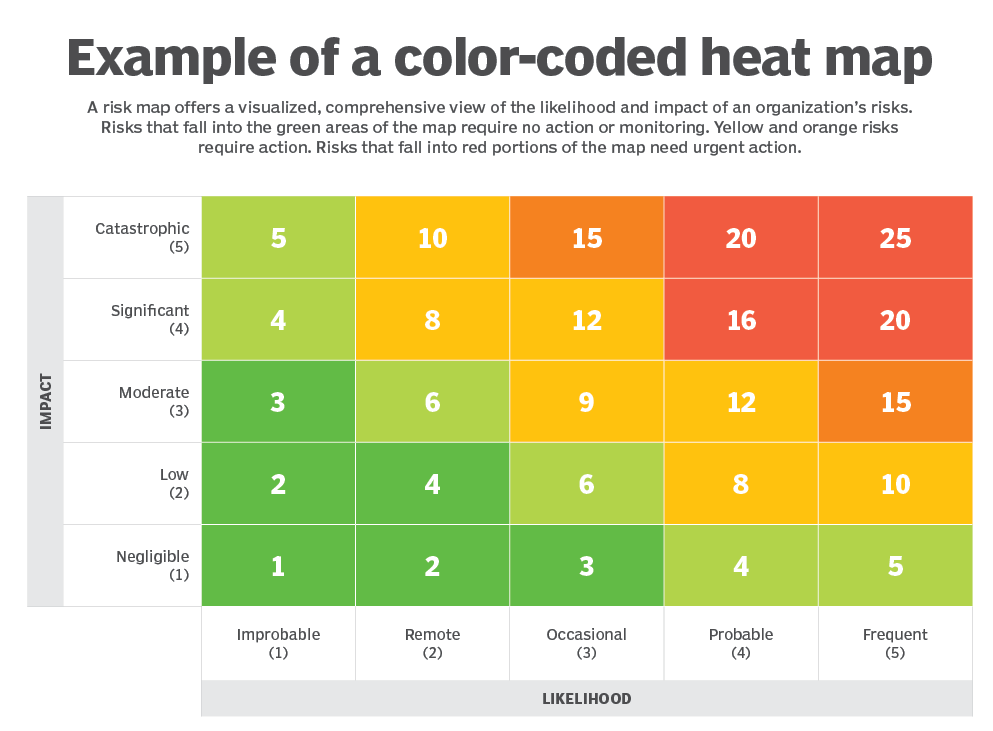
\includegraphics[width=0.8\linewidth]{UNINA_BSc_Final_Report//img//plots/heatmap-example.png} \caption{esempio di heatmap \cite{heatmap-example}} \label{fig:plot-heatmap-example}
\end{figure}

\subsection{Risultati}
Lavorando solo su un subset non è stato ovviamente possibile effettuare un'analisi completa, ma il processo utilizzato è facilmente estendibile a qualsiasi altra metrica.
Le metriche a disposizione sono circa 50, di cui diverse sono risultate essere non indicatrici di un \textbf{comportamento anomalo} come nel caso del ratio dei context switch al secondo dei processi nel nodo master [fig. \ref{fig:plot-useless-example}], dove non si osservano variazioni significative nell'intervallo interquartile (IQR), e le piccole variazioni presenti nei \textit{whisker} potrebbero essere influenzate da fattori esterni alla campagna di injection. \\
Di seguito verranno approfondite le metriche principali che hanno rilevato un comportamento anomalo per i possibili errori di orchestrazione confrontandole con il comportamento medio, che quindi possano effettivamente essere utilizzate per l'alerting o che quantomeno siano utili da monitorare.

\begin{figure} [ht]
    \centering
    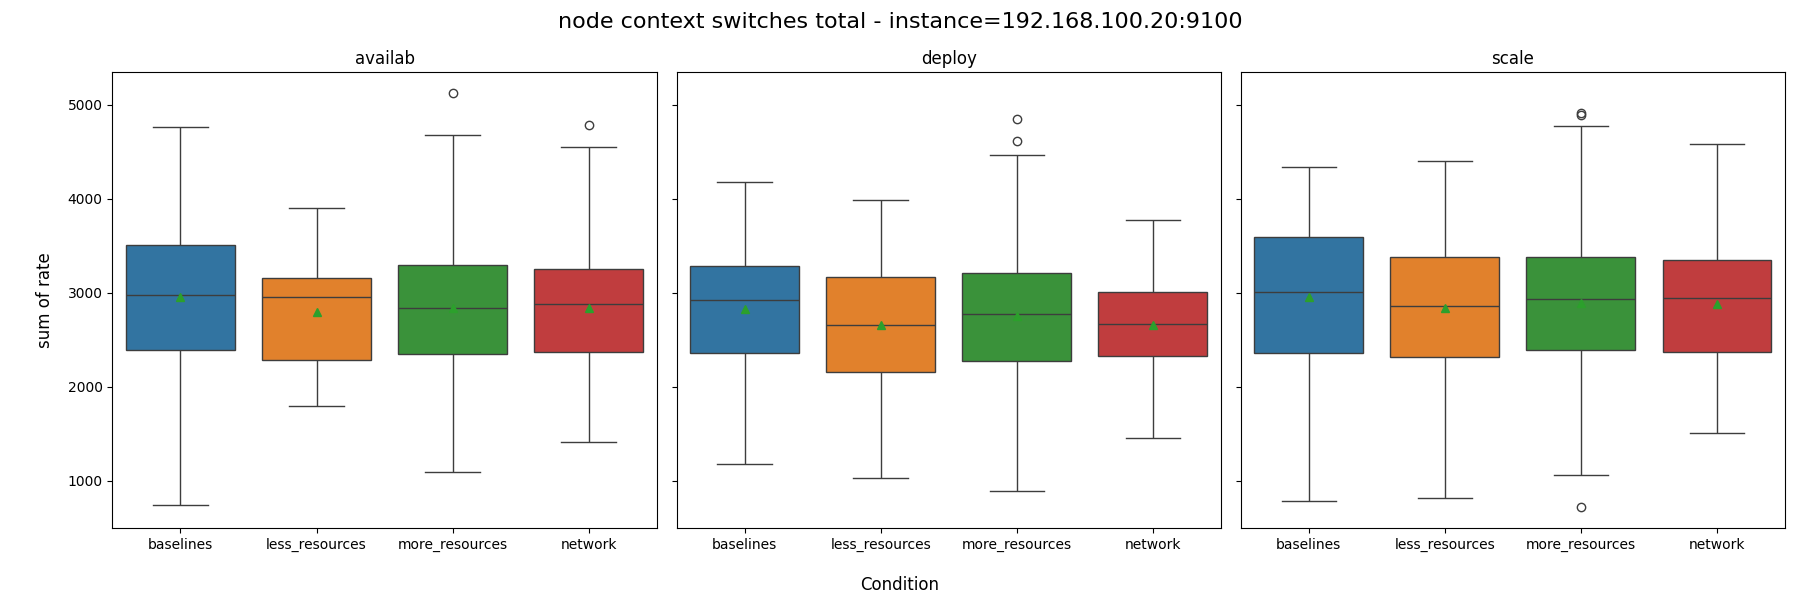
\includegraphics[width=1\linewidth]{UNINA_BSc_Final_Report//img//plots/node context switch - useless example.png}
    \caption{esempio di metrica non rilevante}
    \label{fig:plot-useless-example}
\end{figure}

\subsubsection{Utilizzo risorse}
\begin{figure}
    \centering
    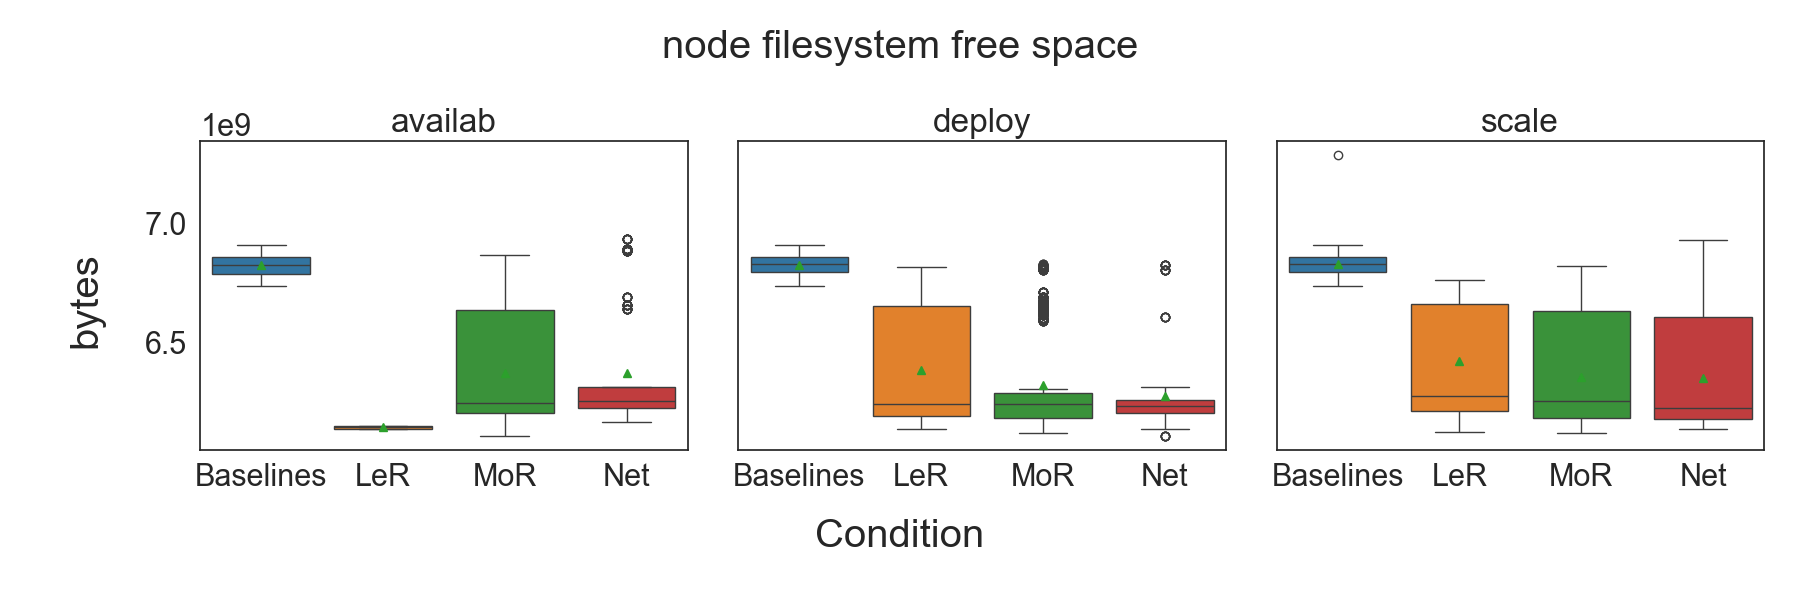
\includegraphics[width=1\linewidth]{UNINA_BSc_Final_Report//img//plots/node_free_fs_space.png}
    \caption{spazio libero del file system sul nodo in bytes \footnotesize(scala 10\(^9\))}
    \label{fig:plot-free-fs}
\end{figure}
Come si può osservare in tutte le condizioni di errore e sotto qualsiasi tipologia di workload, il nodo su cui è installato \textbf{il Control Plane utilizza decisamente più risorse} (circa 1 GB in più, sia sulla partizione del filesystem [fig. \ref{fig:plot-free-fs}] sia sulla memoria [fig. \ref{fig:plot-free-mem}], che su un nodo con 4 GB di ram è decisamente impattante), come si può evincere dal fatto che sotto tutti i workload, per entrambe le metriche, i whisker superiori degli errori non fanno nemmeno parte dell'IQR della baseline oltre ad avere una maggiore dispersione dei dati. Ad esempio il valore medio di memoria libero nel caso LeR sotto worload Availab è stato di circa 0.4 GB, mentre nel caso Baseline è di circa 1.7 GB. Questo probabilmente è il risultato di continue operazioni per cercare di portare lo stato del cluster allo stato desiderato senza mai riuscirci. 
\begin{figure} [!ht]
    \centering
    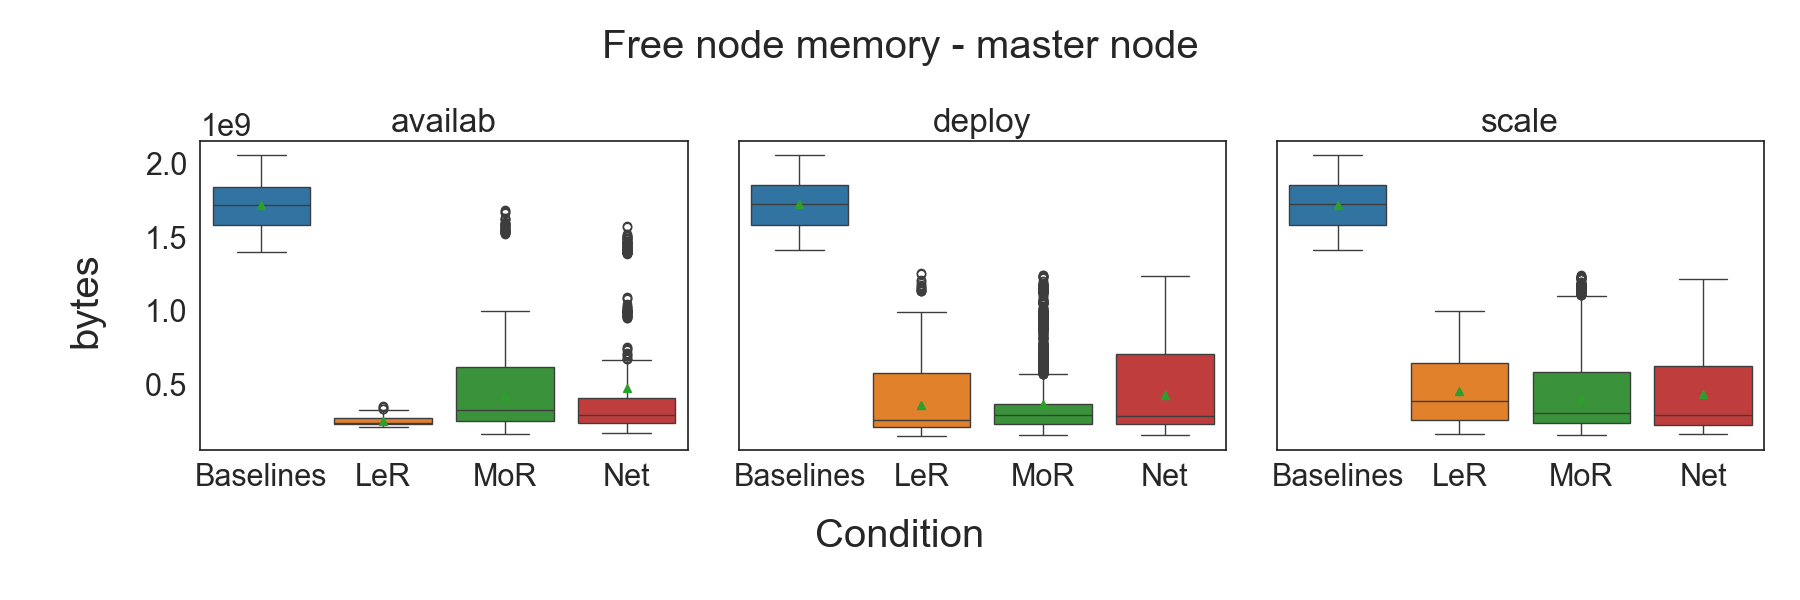
\includegraphics[width=1\linewidth]{node_free_mem.png}
    \caption{spazio libero in memoria sul nodo master in bytes \footnotesize(scala 10\(^9\))}
    \label{fig:plot-free-mem}
\end{figure} \\
In particolare nel caso di errori Net, la memoria disponibile subisce delle forti variazioni perché si verifica una condizione detta \textbf{capacity offset}, in cui la capacità dichiarata di un nodo è diversa dalla capacità effettivamente utilizzabile, a causa delle comunicazioni fallite tra Kubernetes ed il resto del sistema [fig. \ref{fig:plot-mem-net}]. Questa condizione non si verifica nei casi LeR e MoR perché viene proprio modificata la capacità delle risorse dei nodi dichiarata, anche se non corrisponde con l'effettiva capacità delle risorse fisiche del sistema.
\begin{figure}[!ht]
    \centering
    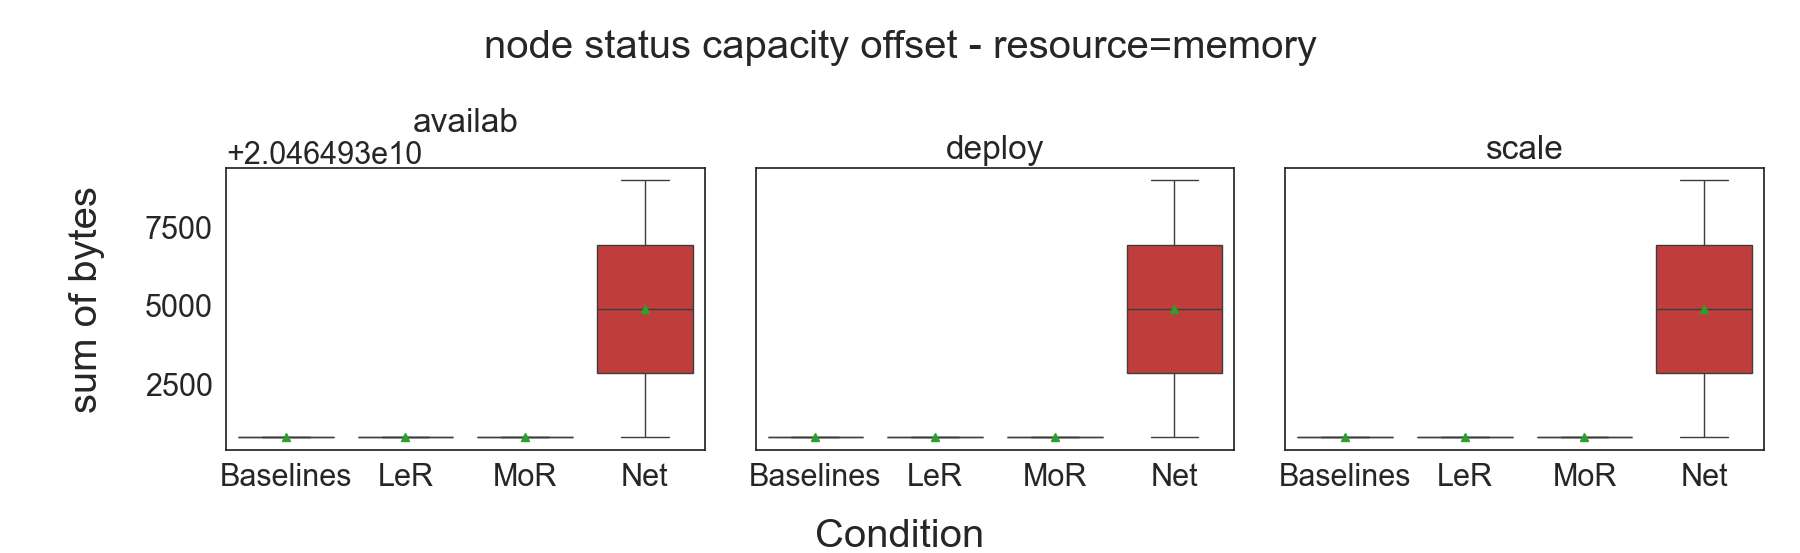
\includegraphics[width=1\linewidth]{UNINA_BSc_Final_Report//img//plots/sum kube_node_status_capacity_offset_offset_time)_by_ resource).png}
    \caption{discrepanza memoria utilizzabile e memoria dichiarata}
    \label{fig:plot-mem-net}
\end{figure}\\ \\ \\ 
Anche il ratio di utilizzo della CPU da parte dei processi può essere un ottimo indicatore, infatti nella condizione MoR si verificano diversi \textbf{picchi}, dove in alcuni casi quasi viene raggiunto il 100\% di utilizzo, indicati dai numerosi outliners, condizione che quindi si è verificata anche relativamente spesso e che può portare al crash dei pod e disservizi agli utenti [fig. \ref{fig:plot-cpu-ratio}].
\begin{figure} [ht]
    \centering
    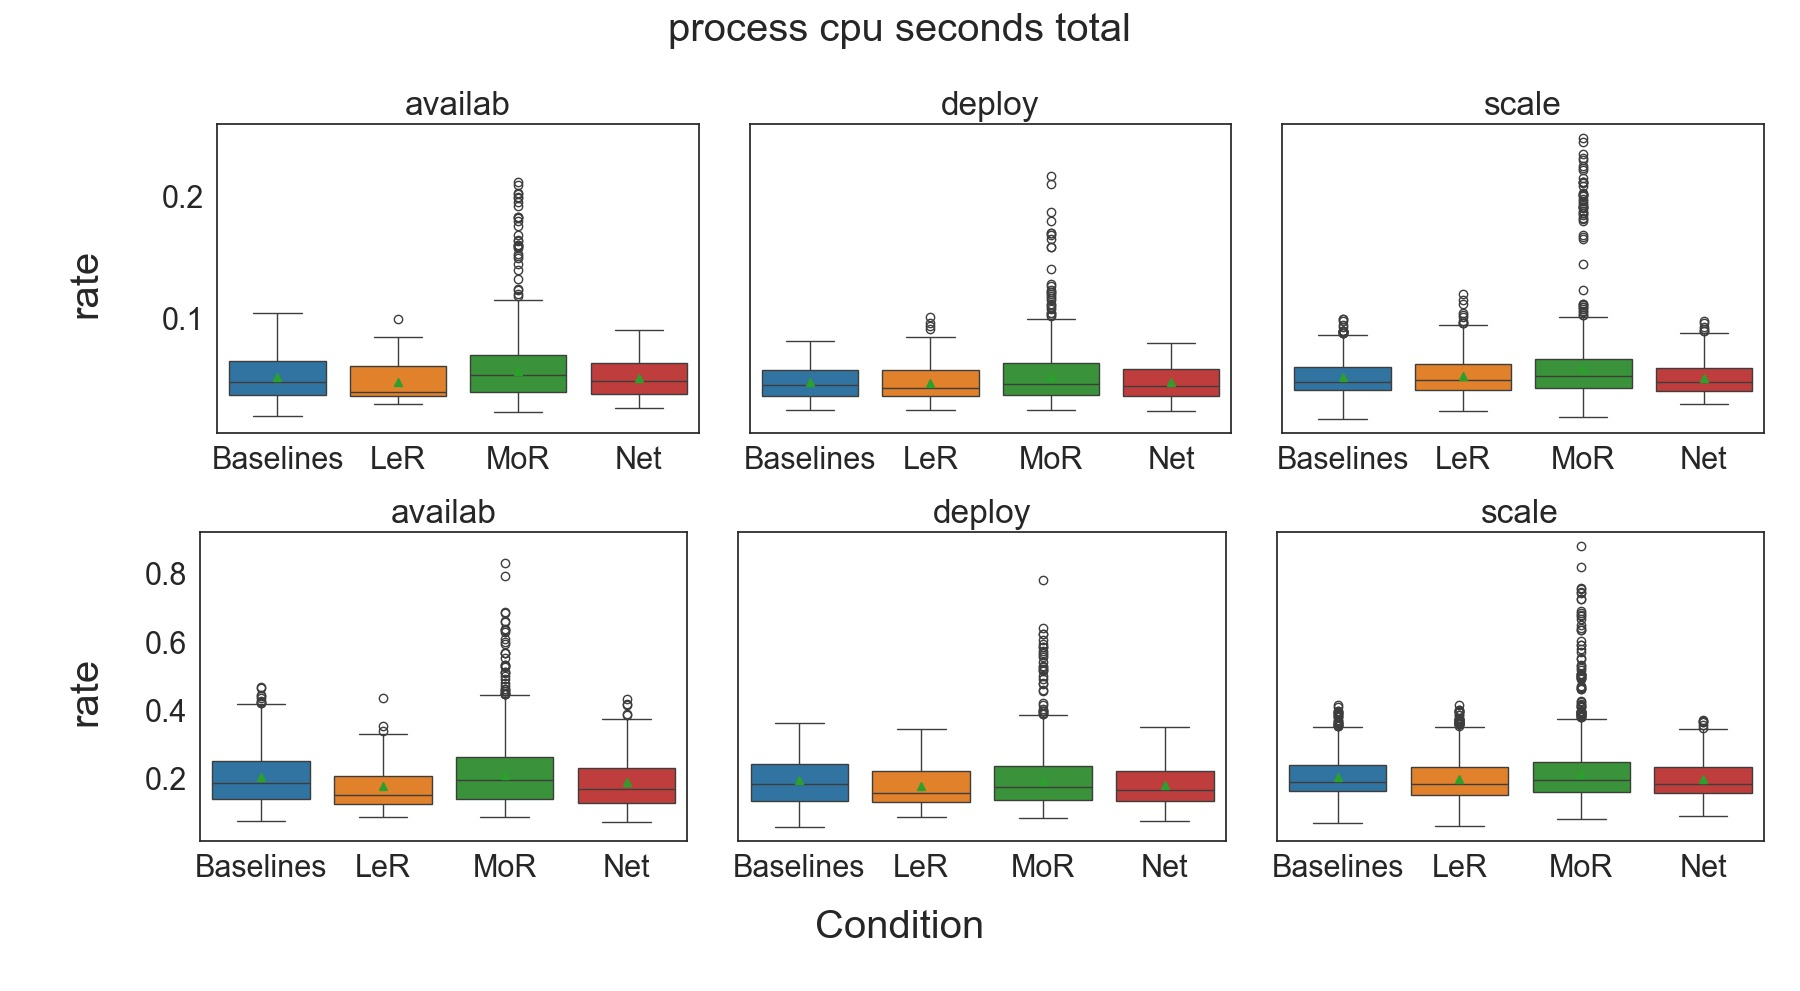
\includegraphics[width=0.8\linewidth]{UNINA_BSc_Final_Report//img//plots/rate process_cpu_seconds_total - all.jpg}
    \caption{ratio utilizzo cpu}
    \label{fig:plot-cpu-ratio}
\end{figure}

\subsubsection{Network}

Un'altra categoria di metriche da tenere sotto controllo riguarda le connessioni tra i nodi. Durante il workload di deploy, ovvero durante la creazione di nuovi pod o altri oggetti in Kubernetes, e in presenza di errori Net, sia il nodo master che i nodi worker tentano di stabilire un \textbf{numero elevato di nuove connessioni}. Questo comportamento si verifica perché molte delle connessioni falliscono, come evidenziato dall'ampiezza dell'intervallo interquartile (IQR) e dalla posizione elevata del whisker superiore. Tale fenomeno è visibile anche nella heatmap delle socket TCP in memoria, dove l'area deploy-Net è più scura rispetto alle altre.
In aggiunta, si osserva un significativo \textbf{incremento del numero di pacchetti inviati}, a cui segue un \textbf{aumento dei pacchetti ritrasmessi} a causa degli errori di comunicazione, chiaramente rilevabile nella heatmap del ratio dei pacchetti ritrasmessi, dove tale area è marcatamente più scura [fig. \ref{fig:plot-net-all}].
\begin{figure} [ht]
    \centering
    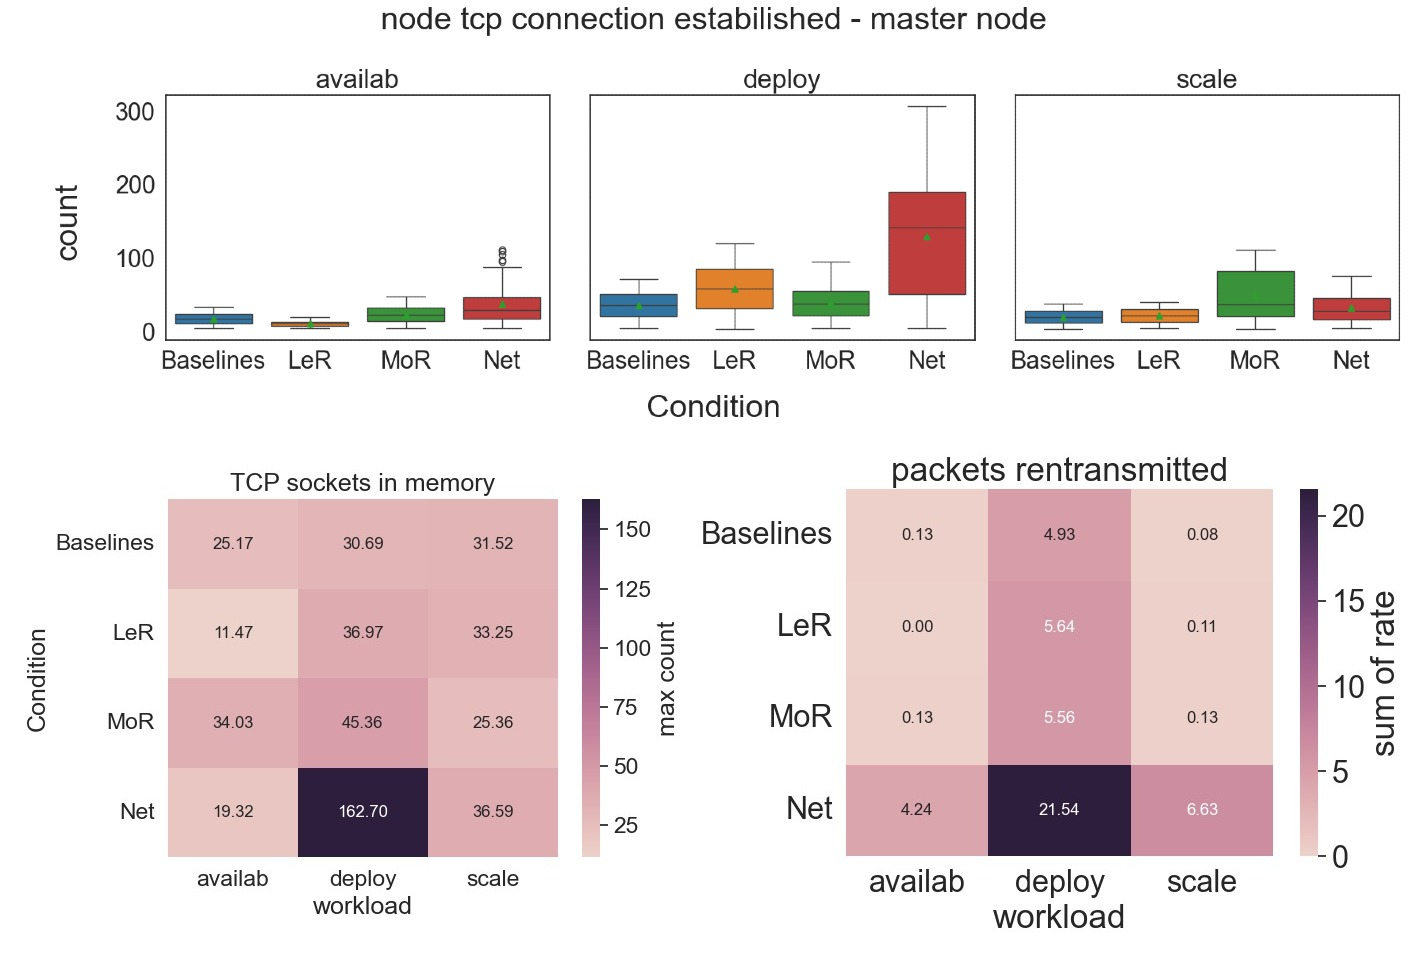
\includegraphics[width=1\linewidth]{UNINA_BSc_Final_Report//img//plots/Network - all.jpg}
    \caption{statistiche metriche di rete}
    \label{fig:plot-net-all}
\end{figure}


\subsubsection{Pod e container}

Lo stato dei pod e dei container va monitorato in maniera tempestiva, dato che sono un ottimo riferimento per controllare la salute dei servizi offerti.
In tutti i casi di errore si può osservare come i container dell'applicazione campione utilizzata nella campagna, \textbf{terminano numerose volte per errori} di diverso tipo, in particolar modo nel caso MoR, questo perché in generale tale problema risulta essere più critico rispetto agli altri dato che vengono assegnate più risorse di quelle disponibili [fig. \ref{fig:plot-pod-container}]. \\
Un altro dettaglio da notare è come nel caso di LeR sotto workload Failover, \textbf{i pod cambiano stato molto meno spesso mentre i container terminati per errore sono decisamente inferiori}, questo proprio perché avendo meno risorse a disposizione vengono creati meno pod e container, quindi una volta che sono stati terminati in maniera forzata molti non vengono più riavviati.
\begin{figure} [ht]
    \centering
    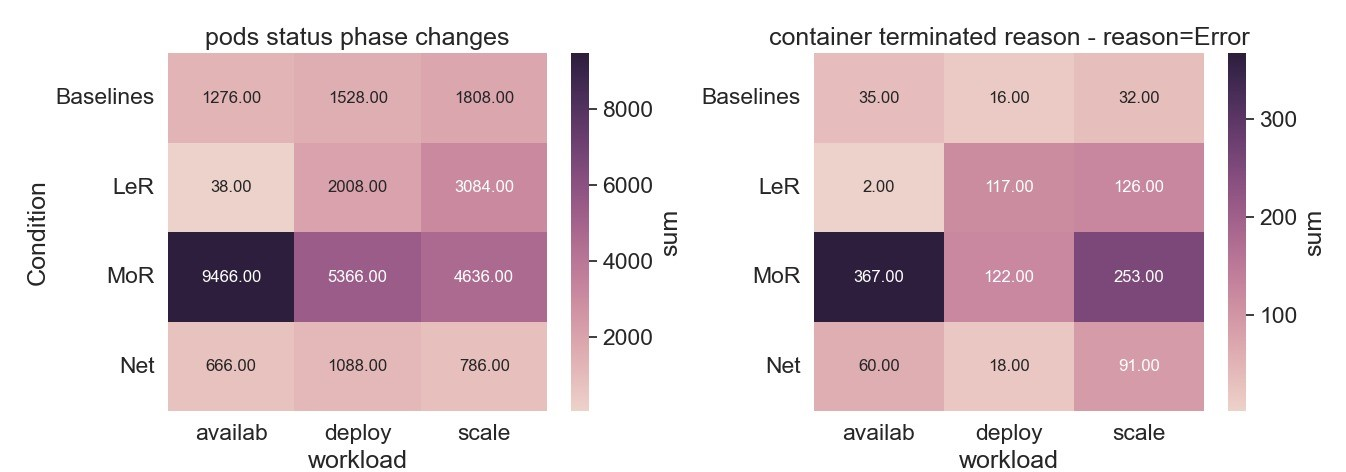
\includegraphics[width=1\linewidth]{UNINA_BSc_Final_Report//img//plots/pods - containers.jpg}
    \caption{variazioni stato pod e container terminati per errore}
    \label{fig:plot-pod-container}
\end{figure}

\subsubsection{Workqueue}

Lo stato delle workqueue permette anch'esso di identificare un eventuale sovraccarico del sistema, come avviene nel caso MoR in cui nelle queue vengono aggiunti spesso \textbf{più task rispetto alla media} [fig. \ref{fig:plot-queue-add}] credendo di avere maggiori risorse computazionali, situazione segnalata dai numerosi outliners, o addirittura nel caso di LeR sotto Failover risultano avere una \textbf{profondità quasi nulla} perché molti dei pod non vengono più riavviati risultando così in un carico molto più basso del normale [fig. \ref{fig:plot-queue-depth}].

\begin{figure} [ht]
    \centering
    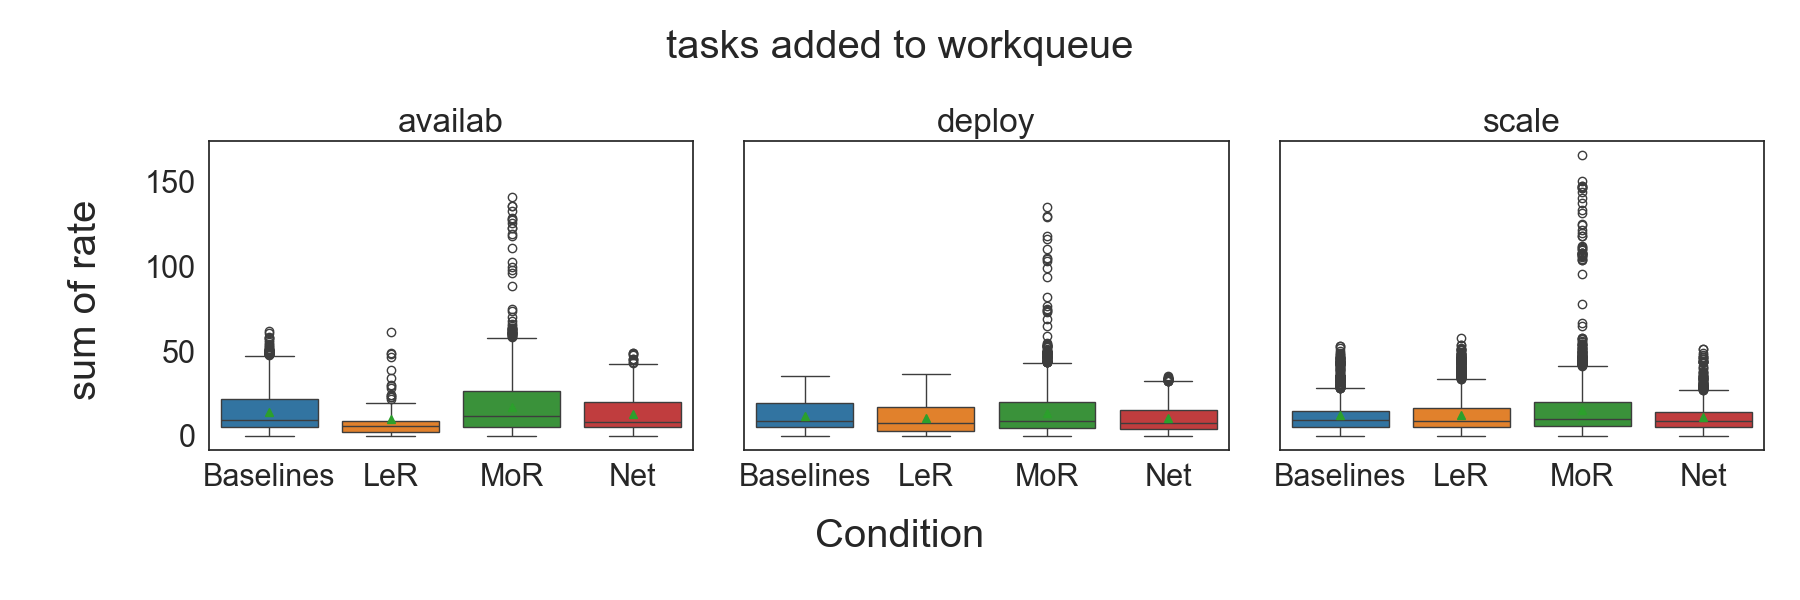
\includegraphics[width=0.9\linewidth]{UNINA_BSc_Final_Report//img//plots/workqueue_adds.png}
    \caption{inserimento task in una workqueue}
    \label{fig:plot-queue-add}
\end{figure}

\begin{figure}
    \centering
    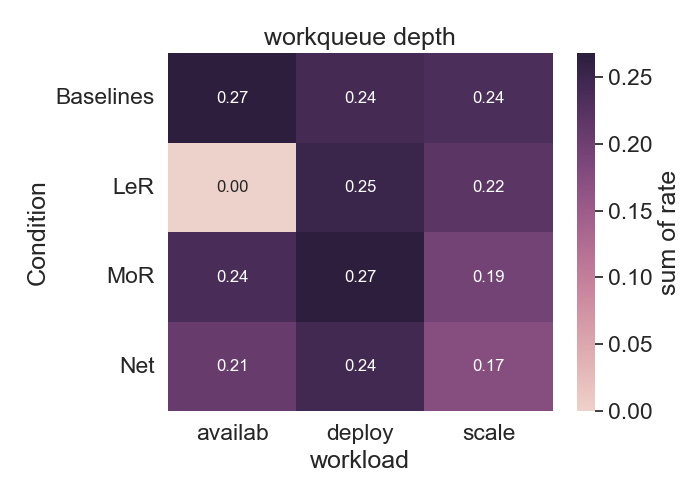
\includegraphics[width=0.5\linewidth]{UNINA_BSc_Final_Report//img//plots/workqueue_depth.png}
    \caption{profondità queue (LeR-Failover quasi nullo)}
    \label{fig:plot-queue-depth}
\end{figure}


\subsubsection{Metriche personalizzate}

Le metriche personalizzate create utilizzando le client library, permettono di monitorare in maniera più approfondita lo stato del servizio offerto, ad esempio con il server Flask utilizzato nella campagna possiamo controllare le \textbf{richieste HTTP ricevute} e relative \textbf{risposte} [fig. \ref{fig:plot-rest-request}]. Controllando ad esempio se in un determinato periodo di tempo le risposte di errore sono superiori alla media dato che nel caso MoR risultano essere particolarmente frequenti, situazione denotabile dai numerosi outliners, a causa del fatto che il BE accetta più richieste di quante possa effettivamente soddisfarne.
\begin{figure} [ht]
    \centering
    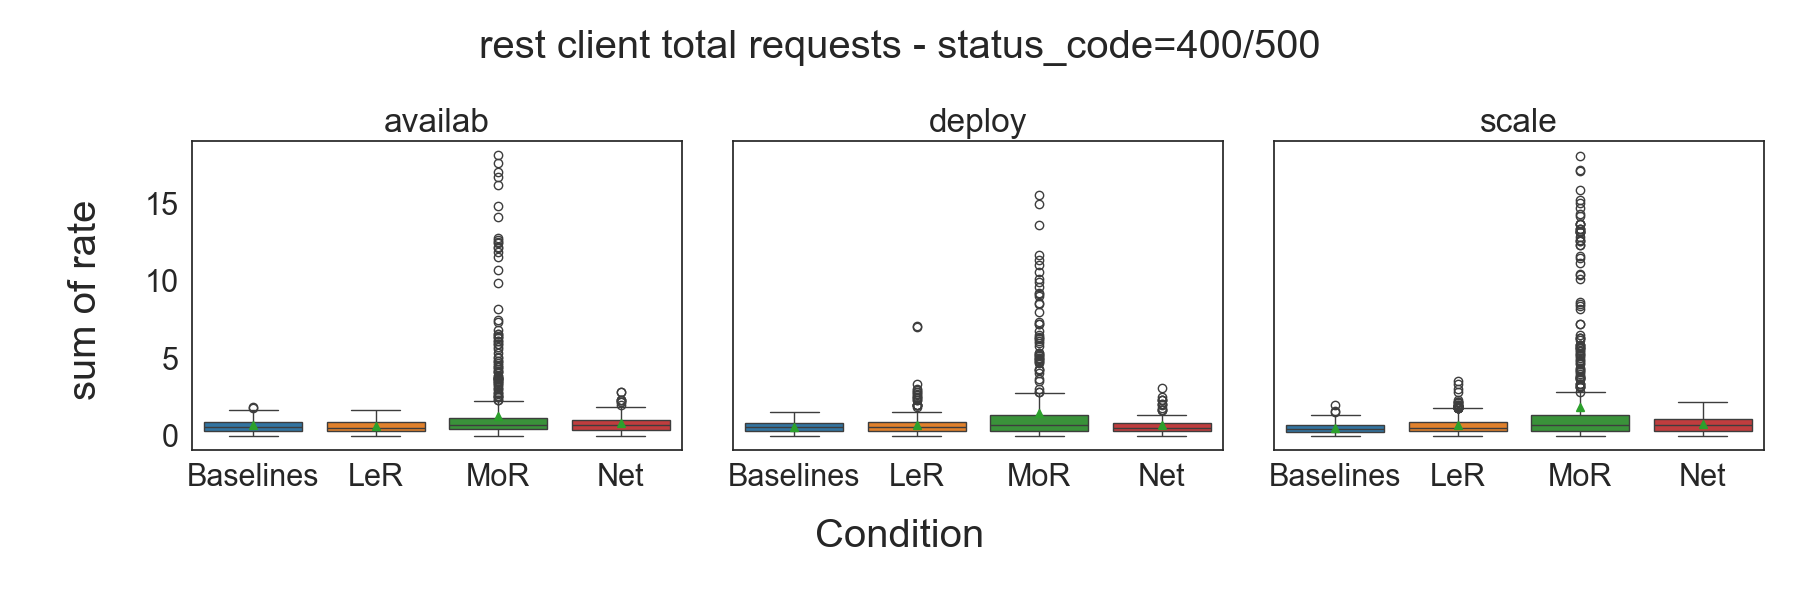
\includegraphics[width=0.9\linewidth]{UNINA_BSc_Final_Report//img//plots/rest requests.png}
    \caption{richieste HTTP con risposta 400/500}
    \label{fig:plot-rest-request}
\end{figure}


\subsection{Utilizzo delle metriche}

Per utilizzare efficacemente le metriche di Prometheus, è innanzitutto necessario ottenere un dataset iniziale che rappresenti lo stato di salute del cluster. Questo consente di stabilire un punto di riferimento per \textbf{identificare eventuali comportamenti anomali}, in maniera simile a quanto fatto precedentemente.\\
Tuttavia, per implementare delle regole di alerting basate su queste metriche, è essenziale definire soglie (\textbf{treshold}) di attivazione appropriate e considerare la possibilità di falsi positivi. Ad esempio, se consideriamo la metrica relativa allo spazio libero in memoria osservato nei nodi [fig. \ref{fig:plot-free-mem}], si può notare che in condizioni normali il nodo master dispone mediamente di circa 1.7 GB di memoria libera, mentre in caso di errore questo valore scende significativamente. Pertanto, si potrebbe impostare una soglia del 15\% inferiore alla media come limite di allerta, utlizzando una query PromQl come: \\
\textbf{\textit{node\_memory\_MemFree\_bytes < THRESHOLD}}
 \\
Con una soglia del 15\%, i falsi positivi risultano essere inferiori all'1\%, mentre il tasso di errori non rilevati è intorno al 2.7\%. Sebbene questi valori siano accettabili, è importante considerare che le variazioni nei dati non sono sempre così evidenti. Ad esempio, nel monitoraggio delle richieste HTTP con status code 400 o 500 [fig. \ref{fig:plot-rest-request}], tali eventi anomali possono essere isolati e limitati a brevi periodi di tempo. Per questo motivo, PromQL consente di \textbf{monitorare le metriche per un intervallo di tempo specifico}, permettendo di verificare, ad esempio, se negli ultimi 3 minuti si è verificato un numero di risposte negative significativamente superiore alla media.\\
\textbf{\textit{sum(rate(rest\_client\_requests\_total\{code=\textasciitilde"[45].."\} [3m] )) > THRESHOLD}}.

\subsection{Riepilogo metriche analizzate}
Le metriche che hanno rilevato un comportamento anomalo in uno o più casi di errore, presenti nel subset analizzato, sono state riepilogate nella tabella in fig. \ref{fig:plot-summary}, dove sono mappate le metriche, le tipologie di errore e i workload. Sono state segnate con un tick i casi in cui le metriche risultano essere utili da monitorare e sulla quale eventualmente applicarci regole di alerting. \\
\begin{figure} [ht]
    \centering
    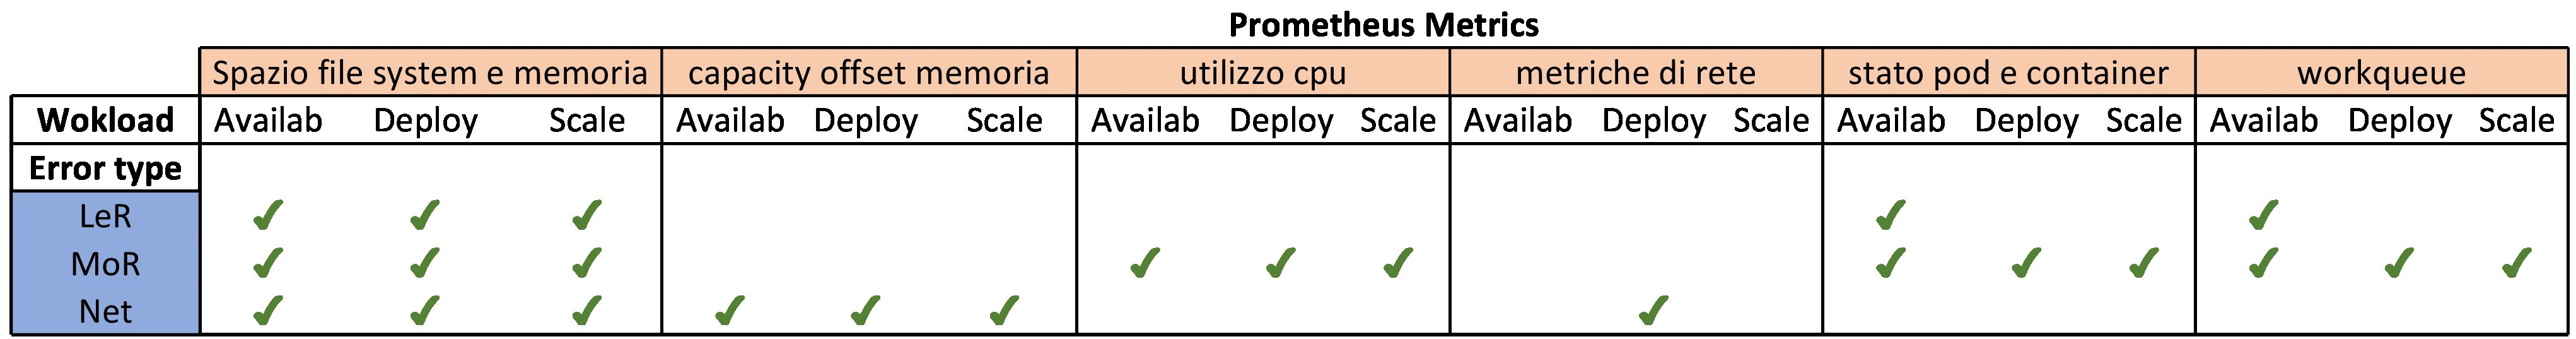
\includegraphics[width=1\linewidth]{UNINA_BSc_Final_Report//img//plots/map-metrics-error-workloads.jpg}
    \caption{mappa riepilogativa metriche - errori - workload}
    \label{fig:plot-summary}
\end{figure}



\chapter{Conclusioni}
Nei moderni sistemi il \textbf{monitoraggio pro-attivo} combinato con il meccanismo di \textbf{alerting} risulta essere un processo di fondamentale importanza che permette di attivarsi repentinamente per risolvere situazioni critiche o fare in modo che non si verifichino. \\
In particolare è stato approfondito \textbf{Prometheus}, un framework che integra entrambe queste tipologie di processi, permettendo di monitorare l'intero sistema target, a partire dallo stato delle macchine su cui viene eseguito, nonché lo stato di uno o più cluster Kubernetes e dei relativi oggetti o monitorare un'applicazione in maniera più dettagliata utilizzando le apposite client library. \\
I dati raccolti durante il monitoraggio sono salvati in maniera \textbf{persistente}, in modo da poterli successivamente utilizzare per effettuare delle \textbf{interrogazioni} tramite l'apposito linguaggio \textbf{PromQL}, che fa da standard per diverse applicazioni di terze parti come Grafana, che permettono di rappresentare i dati in maniera grafica, oppure per l'Alert Manager, con il quale possiamo creare delle apposite \textbf{regole di alerting} come ad esempio per l'eccessivo utilizzo delle risorse negli ultimi minuti. \\
Sfruttando alcune delle metriche messe a disposizione da Prometheus durante la campagna di fault / error injection del progetto Mutiny, è stato osservato come avendo la possibilità di monitorare un ampio spettro di risorse, sia possibile riuscire a verificare quando una delle possibili condizioni di errore stia per verificarsi, dato che ognuna di esse mostrerà spesso dei \textbf{sintomi} che possono essere utilizzati per l'alerting. \\
Inoltre, è stato possibile effettuare una seconda verifica su uno degli insights del paper \cite{Paper}, ovvero che la condizione \textbf{MoR} risulta essere la \textbf{più problematica} dato che un sovraccarico delle risorse può portare ad un aumento dei costi in un ambiente cloud o a terminarle mandando in crash il sistema, infatti risulta anche essere la condizione che generalmente \textbf{causa più sintomi}.


\bibliography{bibliography}
\bibliographystyle{plain}

\end{document}